\ifx\allfiles\undefined
\documentclass[8pt a4paper, oneside, UTF8]{ctexbook}  % +  这一句是新增加的
\usepackage{amsmath}   % 数学公式
\usepackage[dvipsnames]{xcolor}
\usepackage{amsthm}    % 定理环境
\usepackage{amssymb}   % 更多公式符号
\usepackage{graphicx}  % 插图
\usepackage{mathrsfs}  % 数学字体
\usepackage{enumitem}  % 列表
\usepackage{geometry}  % 页面调整
\usepackage{unicode-math}
\usepackage{extarrows}
\usepackage{subfigure}
\usepackage{extarrows}
\usepackage{footnote}
\usepackage{svg}
\usepackage[colorlinks,linkcolor=black]{hyperref}
\usepackage{supertabular}
\usepackage{tcolorbox}
\usepackage{ulem}
\usepackage{framed}
\usepackage{float}
\usepackage{microtype}
\newcommand{\arccot}{\mathrm{arccot}\,}
\tcbuselibrary{breakable}
\tcbuselibrary{most}
\newcounter{problemname}
\newenvironment{solution}{\par\noindent\textbf{解答. }}{\par}
\newenvironment{note}{\par\noindent\textbf{题目\arabic{problemname}的注记. }}{\par}
\definecolor{shadecolor}{RGB}{241, 241, 255}
\newenvironment{problem}{\begin{shaded}\stepcounter{problemname}\par\noindent\textbf{题目\arabic{problemname}. }}{\end{shaded}\par}

\graphicspath{ {figure/},{../figure/}, {config/}, {../config/} }  % 配置图形文件检索目录
\linespread{1.2} % 行高

% 页码设置
\geometry{top=25.4mm,bottom=25.4mm,left=20mm,right=20mm,headheight=2.17cm,headsep=4mm,footskip=12mm}

% 设置列表环境的上下间距
\setenumerate[1]{itemsep=5pt,partopsep=0pt,parsep=\parskip,topsep=5pt}
\setitemize[1]{itemsep=5pt,partopsep=0pt,parsep=\parskip,topsep=5pt}
\setdescription{itemsep=5pt,partopsep=0pt,parsep=\parskip,topsep=5pt}

% 定理环境
% ########## 定理环境 start ####################################

% #### 将 config.tex 中的定理环境的对应部分替换为如下内容
% 定义单独编号,其他四个共用一个编号计数 这里只列举了五种,其他可类似定义(未定义的使用原来的也可)
\newtcbtheorem[auto counter, number within=section, list type=subsubsection, list inside=toc]{defn}{定义}
{
    colback=green!5,colframe=green!35!black,fonttitle=\bfseries, title={Comment \thetcbcounter}, list entry={Comment \thetcbcounter\quad}, %标题
    breakable, %支持跨页
    before upper={\parindent10pt\noindent},  % 支持缩进。\noindent:首行不缩进
    % left = 2mm, %文字离线框左边的边距
    % right = 1mm,%同上
    % top = 1mm,%同上
    % bottom = 1mm,%同上
    % arc is angular = 1mm, % 棱角线框
    % sharp corners, % 直角线框
    % enhanced,frame hidden, % 隐藏线框
    % enhanced, drop fuzzy shadow,  % 显示阴影
}
{def}

\newtcbtheorem[auto counter, number within=section, list type=subsubsection, list inside=toc]{lemma}{引理}
{
    colback=SeaGreen!10!CornflowerBlue!10,colframe=RoyalPurple!55!Aquamarine!100!,fonttitle=\bfseries, title={Comment \thetcbcounter}, list entry={Comment \thetcbcounter\quad}, %标题
    breakable, %支持跨页
    before upper={\parindent10pt\noindent},  % 支持缩进。\noindent:首行不缩进
    % left = 2mm, %文字离线框左边的边距
    % right = 1mm,%同上
    % top = 1mm,%同上
    % bottom = 1mm,%同上
    % arc is angular = 1mm, % 棱角线框
    % sharp corners, % 直角线框
    % enhanced,frame hidden, % 隐藏线框
    % enhanced, drop fuzzy shadow,  % 显示阴影
}
{lem}


\newtcbtheorem[auto counter, number within=section, list type=subsubsection, list inside=toc]{them}{定理}
{
    colback=Salmon!20, colframe=Salmon!90!Black,fonttitle=\bfseries, title={Comment \thetcbcounter}, list entry={Comment \thetcbcounter\quad}, %标题
    breakable, %支持跨页
    before upper={\parindent10pt\noindent},  % 支持缩进。\noindent:首行不缩进
    % left = 2mm, %文字离线框左边的边距
    % right = 1mm,%同上
    % top = 1mm,%同上
    % bottom = 1mm,%同上
    % arc is angular = 1mm, % 棱角线框
    % sharp corners, % 直角线框
    % enhanced,frame hidden, % 隐藏线框
    % enhanced, drop fuzzy shadow,  % 显示阴影
}
{them}
\newtcbtheorem[auto counter, number within=section, list type=subsubsection, list inside=toc]{criterion}{注}
{
    colback=CornflowerBlue!10,colframe=RoyalPurple!55!Aquamarine!100!,fonttitle=\bfseries, title={Comment \thetcbcounter}, list entry={Comment \thetcbcounter\quad}, %标题
    breakable, %支持跨页
    before upper={\parindent10pt\noindent},  % 支持缩进。\noindent:首行不缩进
    % left = 2mm, %文字离线框左边的边距
    % right = 1mm,%同上
    % top = 1mm,%同上
    % bottom = 1mm,%同上
    % arc is angular = 1mm, % 棱角线框
    % sharp corners, % 直角线框
    % enhanced,frame hidden, % 隐藏线框
    % enhanced, drop fuzzy shadow,  % 显示阴影
}
{cri}

\newtcbtheorem[auto counter, number within=section, list type=subsubsection, list inside=toc]{corollary}{推论}
{
    colback=Emerald!10,colframe=cyan!40!black,fonttitle=\bfseries, title={Comment \thetcbcounter}, list entry={Comment \thetcbcounter\quad}, %标题
    breakable, %支持跨页
    before upper={\parindent10pt\noindent},  % 支持缩进。\noindent:首行不缩进
    % left = 2mm, %文字离线框左边的边距
    % right = 1mm,%同上
    % top = 1mm,%同上
    % bottom = 1mm,%同上
    % arc is angular = 1mm, % 棱角线框
    % sharp corners, % 直角线框
    % enhanced,frame hidden, % 隐藏线框
    % enhanced, drop fuzzy shadow,  % 显示阴影
}
{cor}
% colback=red!5,colframe=red!75!black

% ######### 定理环境 end  #####################################

% ↓↓↓↓↓↓↓↓↓↓↓↓↓↓↓↓↓ 以下是自定义的命令  ↓↓↓↓↓↓↓↓↓↓↓↓↓↓↓↓

% 用于调整表格的高度  使用 \hline\xrowht{25pt}
\newcommand{\xrowht}[2][0]{\addstackgap[.5\dimexpr#2\relax]{\vphantom{#1}}}

% 表格环境内长内容换行  
\newcommand{\tabincell}[2]{\begin{tabular}{@{}#1@{}}#2\end{tabular}}

% 使用\linespread{1.5} 之后 cases 环境的行高也会改变,重新定义一个 ca 环境可以自动控制 cases 环境行高
\newenvironment{ca}[1][1]{\linespread{#1} \selectfont \begin{cases}}{\end{cases}}
% 和上面一样
\newenvironment{vx}[1][1]{\linespread{#1} \selectfont \begin{vmatrix}}{\end{vmatrix}}

\def\d{\textup{d}} % 直立体 d 用于微分符号 dx
\def\R{\mathbb{R}} % 实数域
\newcommand{\bs}[1]{\boldsymbol{#1}}    % 加粗,常用于向量
\newcommand{\ora}[1]{\overrightarrow{#1}} % 向量

% 数学 平行 符号
\newcommand{\pll}{\kern 0.5em/\kern -0.8em /\kern 0.5em}

% 用于空行\myspace{1} 表示空一行 填 2 表示空两行  
\newcommand{\myspace}[1]{\par\vspace{#1\baselineskip}}

\begin{document}
\begin{sloppypar}
    % \title{{\Huge{\textbf{高等数学笔记}}}}
\author{作者:于家崇}
\date{\today}
\maketitle                   % 在单独的标题页上生成一个标题

\thispagestyle{empty}        % 前言页面不使用页码
\begin{center}
	\Huge\textbf{前言}
\end{center}

If a job is worth doing,it's worth doing well
\begin{flushright}
	\begin{tabular}{c}
		\today \\ 如果一件事值得去做,那就值得去做好
	\end{tabular}
\end{flushright}

\newpage                      % 新的一页
\pagestyle{plain}             % 设置页眉和页脚的排版方式(plain:页眉是空的,页脚只包含一个居中的页码)
\setcounter{page}{1}          % 重新定义页码从第一页开始
\pagenumbering{Roman}         % 使用大写的罗马数字作为页码
\tableofcontents              % 生成目录

\newpage                      % 以下是正文
\pagestyle{plain}
\setcounter{page}{1}          % 使用阿拉伯数字作为页码
\pagenumbering{arabic}
% \setcounter{chapter}{-1}    % 设置 -1 可作为第零章绪论从第零章开始 
    \else
    \fi
    %  ############################ 正文部分
    \chapter{导数}
    \section{导数的概念}
    \subsection{导数的定义}
    \begin{defn}{导数的定义}{}
        设函数$y=f(x)$在点 $x_0$的某个邻域内有定义,当自变量 $x$ 在 $x_0$处取得增量 $\Delta x$(点$x_0+\Delta x$仍在该邻域内)时,相应地,因变量取得增量$\Delta y=f(x_0+\Delta x)-f(x_0)$;如果$\Delta  y$与$\Delta x$之比当 $\Delta x \to 0$时的极限存在,那么称函数 $y=f(x)$在点 $x_0$处可导,并称这个极限为函数 $y=f(x)$在点 $x_0$处的\textbf{导数},记为$f^{\prime}(x_0)$,即
        $$
            f^{'}(x_{0})=\lim_{x\to x_{0}}\frac{f(x)-f(x_{0})}{x-x_{0}}=\lim_{\Delta x\to0}\frac{\Delta y}{\Delta x}=\lim_{\Delta x\to0}\frac{f(x_{0}+\Delta x)-f(x_{0})}{\Delta x}
        $$
        也可记作$\left.y^{\prime}\right|_{x=x_{0}},\left.\dfrac{\mathrm{d}y}{\mathrm{d}x}\right|_{x=x_{0}}\text{或}\left.\dfrac{\mathrm{d}f(x)}{\mathrm{d}x}\right|_{x=x_{0}}.$
    \end{defn}
    \begin{criterion}{导数定义的注意事项}{}
        \begin{enumerate}
            \item 在考题中,增量$\Delta x$一般会被命题人广义化为"$\square$",即
                  $$
                      f'(x_0)=\lim_{\Delta x \to 0}\frac{f(x_0+\Delta x)-f(x_0)}{\Delta x}\xlongequal{\text{广义化}} \lim_{ \square \to 0}\frac{f(x_0 + \square)-f(x_0)}{\square}
                  $$
                  需要知道的是$\square$需要同时趋近于$0^+$和$0^-$该点导数才存在,如果仅趋近于其中的一个,则是$\square$处的单侧导数\\
                  若在上式中,令$x_0+\Delta x=x$,则可将导数定义式写成
                  $$
                      f^{\prime}(x_{0})=\lim_{x\to x_{0}}\dfrac{f\left(x\right)-f\left(x_{0}\right)}{x-x_{0}}
                  $$
                  观察上式,可以观察到上式有以下特点:
                  \begin{itemize}
                      \item 分母同时趋近于$0^+$和$0^-$
                      \item $\Delta x$在趋于0的过程中没有间断点
                      \item 分子为一个动点一个定点
                  \end{itemize}
            \item 以下的三种说法是等价的:
                  \begin{itemize}
                      \item  $y=f\left(x\right)$在点$x_{0}$处可导
                      \item $y=f\left(x\right)$在点$x_{0}$处导数存在
                      \item  $f^{\prime}\left(x_{0}\right)=A\left(A\text{为有限数}\right)$
                  \end{itemize}
            \item 原函数可导无法推出导函数连续
            \item \textcolor{red}{需要区分一点处的右导数和导数的右极限}
                  \begin{itemize}
                      \item $f_+'(x_0) \Rightarrow$表示一点处的右导数$\Rightarrow \lim_{x \to x_0^+}\dfrac{f(x)-f(x_0)}{x-x_0}$
                      \item $f'(x_0 ^+)=f'(x_0+0) \Rightarrow$导数的右极限$\Rightarrow \lim_{x\to x_0^+}f'(x)$
                      \item $f(x_{0}^{+})=f(x_{0}+0) \Rightarrow$函数的右极限$\Rightarrow \lim_{x\to x ^+ _0}f(x)$
                  \end{itemize}
                  如果函数$f(x)$连续可导或者$f'(x)$连续,那么$f_+'(x_0)=f'(x_0^+)$,即一点处的右导数等于导数的右极限.此处如果可以这样理解:把导数降一个纬度理解,令$f'(x)=F(x)$,那么如果$F(x)$在$x_0$处左侧的值和$F(x)$左侧极限相等,则$F(x)$必须可导或者连续,那么可以得到$f'(x)$连续或$f(x)$连续可导.
                  如果不连续,以函数$f(x)=\begin{cases}
                          x,x \leqslant 0 \\
                          x+1,x >0
                      \end{cases}$为例:
                  显然该函数在$x=0$处不连续.那么:
                  \begin{itemize}
                      \item 左导数:$f_-^{\prime}(0)=\lim_{x\to0^{-}}\dfrac{f(x)-f(0)}{x}=\lim_{x\to0^{-}}\dfrac{x-0}{x}=1$
                      \item 右导数:$f_{+}^{\prime}(0)=\lim_{x\to0}\dfrac{f(x)-f(0)}{x}=\lim_{x\to0^{+}}\dfrac{x+1-0}{x}=\dfrac{1}{0}=\infty $
                      \item 导数的右极限:$\lim_{x \to 0^+}f'(x)=\lim_{x\to 0^+}(x+1)' = 1$
                  \end{itemize}
        \end{enumerate}
    \end{criterion}
    \begin{problem}
    设$f(x)$在$x=0$的某邻域内有定义,并且$|f(x)|\leqslant1-\cos x$,则$f(x)$在$x=0$处:\\
    A:极限存在但不连续 \quad B:连续但不可导 \quad C:可导且$f^\prime(0)=0$ \quad D:可导且$f^\prime(0)\neq0$
    \end{problem}
    \begin{solution}
        由于$\lim_{x\to 0}1-\cos x=0$,由夹逼准则可以得到$\lim_{x\to 0}|f(x)|=0.$将$x=0$代入所给不等式,有$|f(0)|\leqslant 0$,所以$f(0)=0$,那么函数在$x=0$连续.由导数定义得$\lim_{x\to 0}\left|\dfrac{f(x)-f(0)}{x-0}\right|\leqslant \dfrac{1-\cos x}{|x|}=0$.由夹逼准则可以得到$f'(0)=0$
    \end{solution}
    \begin{note}
        本题可能会错误的认为$|f(x)|\leqslant 1-\cos x \to |x|\leqslant 1-\cos x$,然后绘制出一个函数图像,然后就认为B选项是正确的,没有根据题意和导数的定义进行求解.
    \end{note}
    \begin{problem}
    若$f(x)$在点$x_{0}$处的左,右导数都存在,则 $f(x)$在点$x_{0}$处\\
    (A) 可导 \quad (B)连续 \quad  (C)不可导 \quad (D)不一定连续
    \end{problem}
    \begin{solution}
        左右导数存在说明左右可导,左可导说明左连续,右可导说明右连续\footnote{这个地方可以用一点可导的必要条件,将其中的$x \to 0$改写为$x \to 0^-$和$x \to 0^+$,最终可以引申为\textcolor{red}{单侧函数可导 $\to$ 单侧函数连续}}.左连续说明左侧极限等于该点函数值,右连续说明右侧极限等于该点函数值,那么左右极限相等且等于该点函数值,那么函数在该点连续.因此B选项正确.
    \end{solution}
    \begin{problem}
    下列命题正确的个数为:\\
    1.设$\lim_{x\to x_0^-}f^{\prime}(x)$与$\lim_{x\to x_0^+}f^{\prime}(x)$均存在,则 $f(x)$ 在 $x=x_0$ 处必连续\\
    2.设$f^{\prime}_-(x_{0})$与$f^{\prime}_{+}(x_{0})$ 均存在,则$f(x)$在$x=x_{0}$处必连续\\
    3.设$f(x_{0}^{-})$与$f(x_{0}^{+})$均存在,则$f(x)$在$x=x_{0}$处必连续\\
    4.设$\lim_{x\to x_{0}^{-}}f^{\prime}(x)$与$\lim_{x\to x_{0}^{+}}f^{\prime}(x)$中至少有一个不存在,则 $f(x)$ 在 $x=x_0$ 处必不可导
    \end{problem}
    \begin{solution}
        1选项中,$\lim_{x\to x_0^-}f^{\prime}(x)$与$\lim_{x\to x_0^+}f^{\prime}(x)$为导数的左极限和右极限,这两个存在不能说明该点连续.\\
        2选项中,左导数和右导数都存在,则导数存在,则在该点必定连续.\\
        3选项中,函数的左右极限都存在,不能得到该点连续(跳跃间断点)\\
        4选项中,使用逆否命题,本选项写为:若$f(x)$在$x=x_0$处可导,则$\lim_{x\to x_{0}^{-}}f^{\prime}(x)$与$\lim_{x\to x_{0}^{+}}f^{\prime}(x)$都存在.显然$f'(x)$可能振荡,极限不存在.\\
        综上,本题命题正确的个数为1.
    \end{solution}
    \begin{problem}
    设$f(0)=0$,则$f(x)$在点$x=0$可导的充要条件为\\
    (A)$\lim_{h\to0}\dfrac{1}{h^{2}}f(1-\cos h)$存在\quad(B)$\lim_{h\to0}\dfrac{1}{h}f(1-e^h)$ 存在\\
    (C)$\lim_{h\to0}\dfrac1{h^2}f(h-\sin h)$ 存在\quad(D)$\lim_{h\to0}\dfrac{1}{h}[f(2h)-f(h)]$存在
    \end{problem}
    \begin{solution}
        A: $\lim_{h \to 0}\dfrac{f(1 -\cos h)-f(0)}{h^2}=\lim_{h \to 0}\dfrac{f(1-\cos h)-f(0)}{1-\cos h}\cdot \dfrac{1-\cos h}{h^2}$,若$h \to 0$可以知道的是$1- \cos h$趋近于$0^+$,$\dfrac{1 - \cos h}{h^2} \to 1$,那么$\dfrac{1}{2}f_+'(0)$存在\\
        B: $\lim_{h \to 0}\dfrac{1}{h}f(1-e^h)=\lim_{h \to 0}\dfrac{1-e^h}{h}\dfrac{f(1-e^h)-f(0)}{1-e^h}$,易知$1-e^h$同时趋近于$0^+$和$0^-$,那么函数$f'(0)$存在\\
        C:$\lim_{h \to 0}\dfrac{1}{h^2}f(h- \sin h)=\lim_{h\to 0}\dfrac{f(h-\sin h)-f(0)}{h^2}=\lim_{h \to 0}\dfrac{f(h-\sin h)}{h -\sin h}\cdot \dfrac{h-\sin h}{h^2}$,已知$h -\sin h \sim \dfrac{1}{6}h^3$,那么$\lim_{h \to 0}\dfrac{f(h-\sin h)}{h -\sin h}\cdot \dfrac{h}{1}$极限存在,同时$h \to 0$,但是不可以推出$\dfrac{f(h-\sin h)}{h-\sin h}$极限存在,只能得到该极限是为定式,那么更无法推出该导数存在\\
        D:若$\lim_{h \to 0}\dfrac{1}{h}[f(2h)-f(h)]$存在,那么其实什么都推不出来,因为不知道$\dfrac{f(2h)}{h}$和$\dfrac{f(h)}{h}$是否存在,如果写成下列形式$\lim_{h \to 0}\dfrac{[f(2h)-f(0)]-[f(h)-f(0)]}{h}=\lim_{h \to 0}\left(\dfrac{f(2h)-f(0)}{h}-\dfrac{f(h)-f(0)}{h}\right)$,则违反了极限的运算法则.\\
        综上答案选择B选项
    \end{solution}
    \begin{conclusion}{若$f(x)$在$x=0$处可导,则必须满足下面的四个条件:}{}
        \begin{enumerate}
            \item 一动减一定:根据导数定义必须是一个动点减一个定点.比如上题中的D选项,本质上是两个动点相减.
            \item 可正可负:指的是分母,即定义中的$\square$,需要同时趋近于$0^+$和$0^-$,如果只能趋近于一个,则为单侧导数.
            \item 上下同阶:即分子的阶数小于等于分母阶数.但是如果要求是充要条件则必须是同阶.比如下面的例子:
                  若$\lim_{x\to 0}\dfrac{f(x-\sin x)-f(0)}{x^4}$存在,那么$\lim_{x\to 0}\dfrac{f(x-\sin x)-f(0)}{x-\sin x}\cdot \dfrac{x - \sin x}{x^4}$,其中$ x - \sin x \sim \dfrac{1}{6}x^3$,那么$\lim_{x\to 0}\dfrac{f(x-\sin x)-f(0)}{(x-\sin x)-0}\cdot \dfrac{1}{6x}$,其中$\lim_{x\to 0} \dfrac{1}{6x} \to \infty$,那么$\lim_{x\to 0}\dfrac{f(x-\sin x)-f(0)}{(x-\sin x)-0}$必定存在且$\dfrac{f(x-\sin x)-f(0)}{(x-\sin x)-0}=0 \Rightarrow f'(0)=0$
            \item 填满邻域:在定义中的$\square$需要把其附近邻域都给填满.比如下面的例子:$\lim_{n\to \infty}\dfrac{f(\frac{1}{n})-f(0)}{\frac{1}{n}}=0$,无法推出$f'_+(0)=0$存在,因为$\dfrac{1}{n}$取不到无理数,无法包含$\square$邻域
        \end{enumerate}
        上述结论的本质还是导数的定义表达式的特点.
    \end{conclusion}
    \begin{problem}
    设函数$f(x)$连续,且$f'(0)>0$,则存在$\delta >0 $使得:\\
    (A)$f(x)$在$(0,\delta)$内单调增加 \quad (B)$f(x)$在$(0,\delta)$内单调减少\\
    (C)对任意的$x \in (0,\delta)$有$f(x)>f(0)$ \quad    (D)对任意的$x\in (-\delta,0)$有$f(x)>f(0)$
    \end{problem}
    \begin{solution}
        A,B选项:已知函数$f(x)$连续,且函数在$f'(0)$处的导数大于0,那么只能说明函数在$x=0$点导数存在且大于0,0可能是函数的振荡间断点.因此函数无法说明函数在邻域内单增或者单减.C,D选项:对函数在$x=0$求导数,即$\lim_{x\to 0} \dfrac{f(x)-f(0)}{x}>0$,则C选项成立.
    \end{solution}
    \begin{note}
        在本题中,答案给出了一个例子可以满足该题(但是本题中例子并不重要,重要的是思想)即$f\left(x\right)=\left\{\begin{matrix}x+2x^{2}\sin\dfrac{1}{x},&x\neq0,\\0,&x=0,\end{matrix}\right.$,在考研中常用的一个例子是\textcolor{red}{$k \times \sin \dfrac{1}{x^b}\pm M \pm f(x)$}.
    \end{note}
    \begin{lemma}{一点处可导与邻域的关系}{}
        一点可导不可以推出邻域的关系,因此存在振荡间断点.以$f'(x_0)>0$为例,可以得到下面的结论:
        $f'(x_0)>0\begin{cases}
                \nRightarrow \text{邻域内}f'(x)>0 \\
                \nRightarrow \text{邻域内}f(x)\text{单增}
            \end{cases}$
    \end{lemma}
    \begin{criterion}{函数可导性与连续的关系}{}
        \begin{enumerate}
            \item \textcolor{red}{导数若存在,则导数要么连续,要么只可能有振荡间断点}
                  \begin{proof}[导数若存在有振荡间断点的证明:]
                      以函数$F(x)=\begin{cases}
                              x^2 \sin \dfrac{1}{x} ,x \neq 0 \\
                              0,x=0
                          \end{cases}$为例:
                      \\根据导数定义对函数在$x=0$处求导:$F'(0)=\lim_{x\to 0}\dfrac{F(x)-F(0)}{x-0}=\lim_{x\to 0}\dfrac{x^2 \sin \frac1x - 0}{x}=\lim_{x\to 0}x \sin \dfrac{1}{x}=0$因此函数$F(x)$在$x=0$处导数存在.那么对函数求导:\\
                      $F'(x)=\begin{cases}
                              2x \sin \dfrac{1}{x} -\cos \dfrac{1}{x} ,x\neq 0 \\
                              0 ,x=0
                          \end{cases}$,那么易知$\lim_{x\to 0}\left(2 x \sin \dfrac{1}{x} -\cos \dfrac{1}{x} \right)$是振荡的.虽然函数导数存在,但是这是振荡间断点.
                  \end{proof}
                  上述推论还可以用几何来解释.如果$x=0$处的导数存在,那么其函数图像在原点一定有切线.
                  \begin{figure}[H]
                      \begin{minipage}[t]{0.5\linewidth}
                          \centering
                          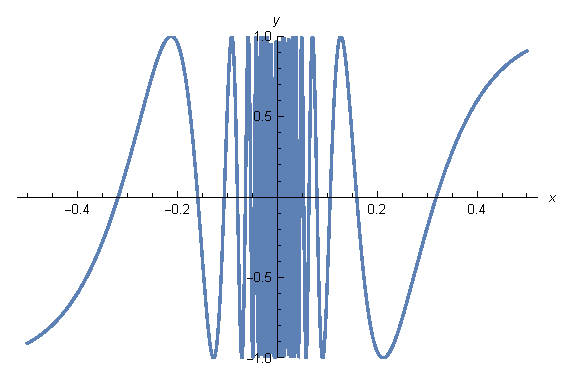
\includegraphics[height=4cm,width=4cm]{3.2.3.eps}
                          \caption{振荡间断点函数$\sin \dfrac{1}{x}$图像}
                      \end{minipage}%
                      \begin{minipage}[t]{0.5\linewidth}
                          \centering
                          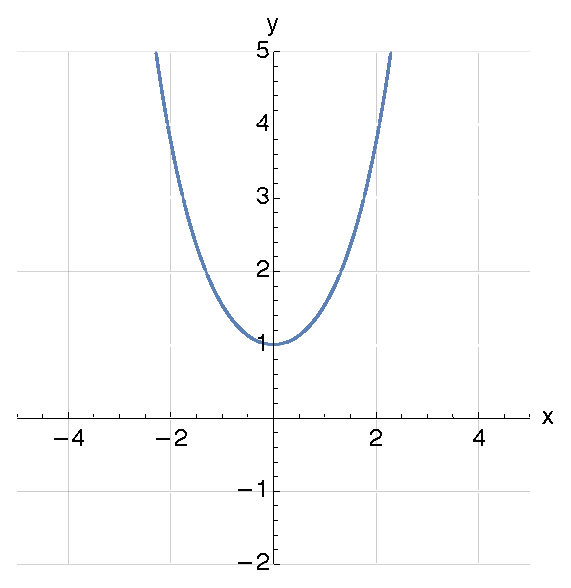
\includegraphics[height=4cm,width=4cm]{1.2.2.eps}
                          \caption{双曲余弦函数$y=\dfrac{e^x+e^{-x}}{2}$}
                      \end{minipage}
                  \end{figure}
                  同时,导数振荡的话,则导数极限不存在,由此可以推出衍生推论:导数极限定理\ref{dsjxdl}
            \item 导数极限如果存在,则导数一定连续(排除了振荡间断点的情况).
            \item \textcolor{red}{函数在一点可导的必要条件:若$f(x)$在一点可导,则$f(x)$在该点连续}\footnote{上面两个结论非常重要,经常和高阶导数一起考察}
        \end{enumerate}
    \end{criterion}
    \begin{problem}
    \getRating{1}已知函数$f(x)\:=\begin{cases}
            x,            & x\leqslant0,                                           \\
            \dfrac{1}{n}, & \dfrac{1}{n+1} < x \leq \dfrac{1}{n},n\:=\:1,2,\cdots,\end{cases}$则:\\
    (A)$x=0$ 是$f(x)$ 的第一类间断点. \quad (C)$f(x)$在$x=0$处连续但不可导.\\
    (B) $x$ = 0 是$f(x)$ 的第二类间断点.\quad (D)$f(x)$在$x=0$处可导.
    \end{problem}
    \begin{solution}
        AB:对$x=0$处求导数,$\lim_{x\to 0^-}f(x)=\lim_{x\to 0^-}x=0$,$\lim_{x\to 0^+}f(x)=\lim_{n\to \infty}\dfrac{1}{n}=0$,则$f(x)$在$x=0$连续,不存在间断点.\\
        CD:对$f_-'(0)=\lim_{x\to 0^-}\dfrac{f(x)-f(0)}{x}=\lim_{x\to 0^-}\dfrac{x}{x}=1$,$f_+'(0)=\lim_{x\to 0^+}\dfrac{f(x)-f(0)}{x}=\lim_{n\to \infty}\dfrac{\frac{1}{n}}{x},\dfrac{1}{n+1}<x \leqslant \dfrac{1}{n}$,由夹逼准则可以得到,$f_+'(0)=1$,$f'(0)=1$\\
        综上,本题应选择D选项.
    \end{solution}
    \begin{note}
        在此题中,$f_{+}^{\prime}(0)=\lim_{\frac{1}{n}\to0^{+}}\dfrac{f\left(0+\frac{1}{n}\right)-f\left(0\right)}{\frac{1}{n}}$,这样写是正确的,因为已经通过证明证得$f'(0)$存在,因此可以这样写.但是一般情况下,$f_{+}^{\prime}(0) \xlongequal{\text{并不一定}}\lim_{\frac{1}{n}+0^{+}}\dfrac{f\left(0+\frac{1}{n}\right)-f\left(0\right)}{\frac{1}{n}}.$因为$n$为正整数,导致区间不能完全覆盖,因此不一定能做到等价,除非证明该点导数存在.此外,不能通过判断$x>0$时图像的存在性来判断该点是否可导.
    \end{note}
    \begin{them}{导数极限定理}{}\label{dsjxdl}
        如果$f(x)$在$x_0$的邻域内连续,在$x_{0}$的去心邻域内可导,且导函数在$x_{0}$处的极限存在(等于$a$),则$f(x)$在$x_0$处的导数也存在并且等于导函数的极限(等于$a$)
    \end{them}
    上述定理可解释为导数如果在某点极限(导数的极限)存在,那么在该点导函数一定连续.因为导数存在要么有振荡间断点,要么连续.如果说该点导函数的极限存在,那么一定连续.
    \begin{problem}
    设$f(x)$ 在 $x=x_0$ 处有二阶导数,则\\
    (A) 当$f(x)$在$x_0$的某邻域内严格单调增加时,$f^\prime(x_0)>0.$
    (B)当$f^\prime(x_0)>0$时,$f(x)$在$x_0$的某邻域内单调增加\\
    (C)当$f(x)$在$x_0$的某邻域内是凹函数时,$f^{\prime\prime}(x_0)>0.$
    (D)当$f^{\prime\prime}(x_0)>0$时,$f(x)$在$x_0$的某邻域内是凹函数
    \end{problem}
    \begin{solution}
        如果该点二阶导数存在,那么该点导数存在且连续.A,C选项错误的原因是未考虑严格单增.B,D选项错误的原因是未考虑振荡间断点.\\
        A:当函数$f(x)$在$x_0$处的邻域内单增,$f'(x_0)$的值可以为0,这样函数也是单调递增.\\
        B:已知$f(x)$ 在 $x=x_0$ 处有二阶导数,那么$f'(x)$在$x_0$处连续.当函数$f'(x_0)>0$时,排除了振荡的情况,因此B选项正确\\
        C:邻域内$f''(x)>0$,则$f(x)$为凹函数,反之则不行,因为可能存在二阶导为0的点,但是依然为凹函数,如$f(x)=x^2$\\
        D:$f''(x_0)>0$可能存在振荡间断点,因此不能推出邻域内$f''(x)>0$
    \end{solution}
    \begin{note}
        D选项,如果增加条件,$f''(x)$在$x=x_0$处连续或$f'''(x_0)$存在,则D选项也成立.\\此外本题应注意两个问题:1.\textcolor{red}{在考虑函数导数存在时,应考虑到振荡间断点和连续的情况}2.\textcolor{red}{在考虑函数在区间内单增和单减时,应考虑是严格单增还是单增.}
    \end{note}
    \begin{problem}
    \getRating{1}已知 $f(x)$ 在 $x=0$ 处连续,且$\lim_{x\to 0}\dfrac{x^2}{f(x)}=1$,则下列结论中正确的个数为\\
    (1)$f^{\prime}(0)$ 存在,且 $f^\prime(0)=0.$ \quad (2)$f^{\prime\prime}(0)$ 存在,且 $f^{\prime\prime}(0)=2.$\\
    (3)$f(x)$在$x=0$处取得极小值\quad (4)$f\left(x\right)$在 $x=0$ 的某邻域内连续.
    \end{problem}
    \begin{solution}
        (1)选项:已知$f(x)$在$x=0$处连续,并且$\lim_{x\to 0}\dfrac{x^2}{f(x)}=1$,则$\lim_{x\to 0}f(x) =0$,由于$f(x)$在$x=0$处连续,那么$\lim_{x \to 0}f(x)=f(0)=0$,导数在$x=0$处的定义式为$\lim_{x\to 0}\dfrac{f(x)-f(0)}{x}=\lim_{x\to 0} \dfrac{f(x)}{x}$.那么$f'(0)=0$\\
        (2)选项:本题无法得到有关二阶导的任何信息.\\
        (3)选项: $\lim_{x\to 0} \dfrac{x^2}{f(x)}=1$,显然$f(x)$在邻域内是大于0的,又因为该点连续,则$x=0$显然为极小值. \\
        (4)选项: 一点可导只能推一点处连续,推不出邻域内连续
    \end{solution}
    \begin{note}
        本题有两个易错点,1:\textcolor{red}{一点可导只能推一点处连续,推不出邻域内连续.}2:\textcolor{red}{只有等价可以替代,极限相等不是等价}.\newline
        此外,在本题的2选项中,有一个易错的思路,即认为一点处的导数($\lim_{x\to 0}\dfrac{f(x)-f(0)}{x}$)=导数的极限($\lim_{x\to 0}f'(x)$),\textcolor{red}{需要注意的是,在极限中,只有等价可以进行替换},例如等价无穷小使用等价替换,即:$1-\cos x \sim \dfrac{1}{2}x^2$,在此题中,$\lim_{x\to 0}\dfrac{f(x)-f(0)}{x} \neq \lim_{x\to 0}f'(x)$,因为二者只是极限相等,极限相等不可以等价.综上,本题正确的个数是2个,分别为1,3选项.
    \end{note}
    \begin{problem}
    \getRating{1}
    设函数$f(x)$在$(-1,1)$上有定义,且$\lim_{x\to0}f(x)=0$,则\\
    (A)当$\lim_{x\to 0}\dfrac{f(x)}{\sqrt{|x|}}=0$时$,f(x)$在$x=0$处可导
    (B)当$\lim_{x\to 0}\dfrac{f(x)}{x^{2}}=0$时$,f(x)$在$x=0$处可导\\
    (C)当$f(x)$在$x=0$处可导时$,\lim_{x\to0}\dfrac{f(x)}{\sqrt{|x|}}=0$\quad
    (D)当$f(x)$在$x=0$处可导时$,\lim_{x\to0}\dfrac{f(x)}{x^{2}}=0$
    \end{problem}
    \begin{solution}
        如果下列选项想在$x=0$处可导,那么$f(0)=0$.\\
        A,B选项无法得到$f(0)=0$\\
        C:$\lim_{x\to 0}\dfrac{f(x)}{\sqrt{|x|}}=\lim_{x\to 0} \dfrac{f(x)}{x}\cdot \dfrac{x}{\sqrt{|x|}}=f'(0)\cdot \dfrac{x}{\sqrt{|x|}}=0$\\
        D:$\lim_{x\to 0}\dfrac{f(x)}{x^2}=\lim_{x\to 0} \dfrac{f(x)}{x}\cdot \dfrac{x}{x^2}=f'(0)\cdot \dfrac{x}{x^2}=\infty$
    \end{solution}
    \begin{note}
        \textcolor{red}{在一元函数中优先看可导推极限},在本题中,CD选项为可导推极限,AB选项为极限推可导.因此应该先看CD选项.此外还应注意 \textcolor{red}{等价替换的使用}
    \end{note}
    \subsection{带绝对值的函数的可导性}
    \begin{itemize}
        \item 可导+可导=可导
        \item 可导+不可导=不可导
        \item 不可导+不可导=无法确定
    \end{itemize}
    \begin{conclusion}{带绝对值函数可导的充要条件}{}
        设 $f(x)=\varphi(x)\left|x-a\right|$,其 $\varphi(x)$ 在$x=a$处连续,则$f\left(x\right)$在$x=a$处可导的充要条件是$\varphi\left(a\right)=0$\footnote{如果该点不可导的话,在$a$点应该函数图像应该由于绝对值的存在,导致存在一个"尖"(绝对值的分段点),最终导致不可导,如果想导,则要在此点可导,整体函数必须为0}
    \end{conclusion}
    \begin{problem}
    设 $f(x)$ 可导$,F(x)=f(x)(1+|\sin x|)$,则 $f(0)=0$ 是$F(x)$ 在$x=0$ 可导的\\
    (A)充分必要条件 \quad (B)充分条件但非必要条件\\
    (C)必要条件但非充分条件 \quad (D)既非充分条件又非必要条件
    \end{problem}
    \begin{solution}
        $F(x)$ 在$x=0$ 的可导性由$f(x)|\sin x|$决定,根据单侧极限定义式
        $$\lim\limits_{x\to0}\frac{\varphi(x)-\varphi(0)}{x-0}=\lim\limits_{x\to0}\frac{f(x)\left|\sin x\right|}{x}=\begin{cases}f(0) ,&x\to0^+\\[2ex]-f(0) ,&x\to0^-\end{cases}$$
        易知$f(0)=0$时$\varphi(x)$在该点连续,则根据结论$\varphi(0)$是充要条件.
    \end{solution}
    \begin{problem}
    函数$f(x)=(x^2-x-2)\mid x^3-x\mid$不可导的点的个数是
    \end{problem}
    \begin{solution}
        $f(x)=(x-2)(x+1)|x+1||x-1||x|$易知$\pm 1,0$为$|x+1||x-1||x|$不可导点.$\varphi(-1) = 0$,因此该点可导.综上,函数不可导点为$1,0$.
    \end{solution}
    \begin{problem}
    设函数$f(x)=\mid x^3-1\mid\varphi(x)$,其中$\varphi(x)$在$x=1$处连续,则$\varphi(1)=0$是$f(x)$在$x=1$处可导的 \\
    (A)充分必要条件 \quad (B)充分条件但非必要条件\\
    (C)必要条件但非充分条件 \quad (D)既非充分条件又非必要条件
    \end{problem}
    \begin{solution}
        $f(x)=|x-1||x^2+x+1|\varphi(x)$,根据结论,显然是充分必要条件.
    \end{solution}
    \begin{problem}
    设 $f(x)$ 在 $x=0$ 的某邻域内有定义, 则 $F(x)=f(x)|\sin x|$ 在 $x=0$ 处可导的充要条件是 ( ).\\
    A. $\lim _{x \rightarrow 0} f(x)$ 存在\\
    B. $\lim _{x \rightarrow 0} f(x)=f(0)$\\
    C. $f(x)$ 在 $x=0$ 处可导\\
    D. $\lim _{x \rightarrow 0^{-}} f(x)$ 与 $\lim _{x \rightarrow 0^{+}} f(x)$ 均存在, 且 $\lim _{x \rightarrow 0^{-}} f(x)=-\lim _{x \rightarrow 0^{+}} f(x)$
    \end{problem}
    \begin{solution}
        由于不知道$f(x)$在该点的连续性,因此不可以使用结论,只能使用导数的定义.当左右导数存在且相等时,函数可导. 即:
        $$
            F_{-}^{\prime}(0)=\lim_{x\to0^{-}}\frac{F(x)-F(0)}{x-0}=\lim_{x\to0^{-}}\frac{-f(x)\sin x}{x}=-\lim_{x\to0^{-}}f(x)
        $$
        $$
            F_{+}^{\prime}(0)=\lim_{x\to0^{+}}\frac{F(x)-F(0)}{x-0}=\lim_{x\to0^{+}}\frac{f(x)\sin x}{x}=\lim_{x\to0^{+}}f(x)
        $$
        综上,应当选择D选项.
    \end{solution}
    \begin{problem}
    设$f(x)$在点$x=a$处可导,则函数$\mid f(x)\mid$在点$x=a$处不可导的充分条件是\\
    (A$)f(a)=0$,且 $f^\prime(a)=0.$ \quad $(C)f(a)>0$,且 $f^\prime(a)>0.$ \\
    (B$)f(a)=0$,且$f^\prime(a)\neq0.$ \quad   (D$)f(a)<0$,且$f^\prime(a)<0.$
    \end{problem}
    \begin{solution}
        根据结论$f(x)$与$|f(x)|$可导性结论\ref{jdzkd},易知B选项正确.CD选项由于该点函数值非0显然使得$|f(x)|$在$x=a$处可导.A选项即使$f(a)$为0,但是由于该点导数为0,可能存在如$x^3$在$x=0$处的情况.
    \end{solution}
    \begin{lemma}{$f(x)$和$|f(x)|$可导性之间的关系}{}\label{jdzkd}
        \begin{itemize}
            \item 两者无任何关系.$f(x)$可导$\nleftrightarrow |f(x)|$可导,但是$f(x)$不可导$\nleftrightarrow |f(x)|$不可导
            \item 设$f(x)$连续
                  \begin{itemize}
                      \item 若 $f\left(x_{0}\right)\neq$0,则 $f\left(x\right)$在 $x_{0}$处可导$\Leftrightarrow\left|f\left(x\right)\right|$在 $x_{0}$ 处可导

                            \tikzset{every picture/.style={line width=0.75pt}} %set default line width to 0.75pt        
                            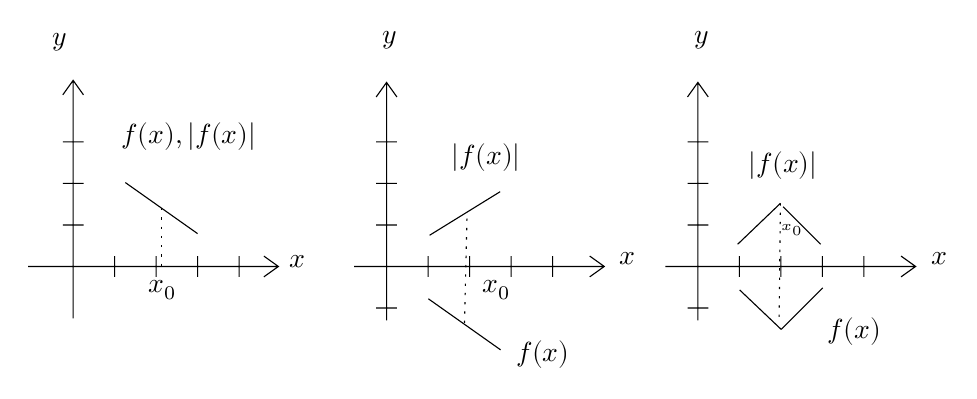
\begin{tikzpicture}[x=0.75pt,y=0.75pt,yscale=-1,xscale=1]
                                \draw  (28.22,199.43) -- (148.75,199.43)(49.86,109.77) -- (49.86,224.43) (141.75,194.43) -- (148.75,199.43) -- (141.75,204.43) (44.86,116.77) -- (49.86,109.77) -- (54.86,116.77) (69.86,194.43) -- (69.86,204.43)(89.86,194.43) -- (89.86,204.43)(109.86,194.43) -- (109.86,204.43)(129.86,194.43) -- (129.86,204.43)(44.86,179.43) -- (54.86,179.43)(44.86,159.43) -- (54.86,159.43)(44.86,139.43) -- (54.86,139.43) ;
                                \draw   ;
                                \draw  (185.22,199.43) -- (305.75,199.43)(200.86,110.77) -- (200.86,225.43) (298.75,194.43) -- (305.75,199.43) -- (298.75,204.43) (195.86,117.77) -- (200.86,110.77) -- (205.86,117.77) (220.86,194.43) -- (220.86,204.43)(240.86,194.43) -- (240.86,204.43)(260.86,194.43) -- (260.86,204.43)(280.86,194.43) -- (280.86,204.43)(195.86,179.43) -- (205.86,179.43)(195.86,159.43) -- (205.86,159.43)(195.86,139.43) -- (205.86,139.43)(195.86,219.43) -- (205.86,219.43) ;
                                \draw   ;
                                \draw  (335.22,199.43) -- (455.75,199.43)(350.86,110.77) -- (350.86,225.43) (448.75,194.43) -- (455.75,199.43) -- (448.75,204.43) (345.86,117.77) -- (350.86,110.77) -- (355.86,117.77) (370.86,194.43) -- (370.86,204.43)(390.86,194.43) -- (390.86,204.43)(410.86,194.43) -- (410.86,204.43)(430.86,194.43) -- (430.86,204.43)(345.86,179.43) -- (355.86,179.43)(345.86,159.43) -- (355.86,159.43)(345.86,139.43) -- (355.86,139.43)(345.86,219.43) -- (355.86,219.43) ;
                                \draw   ;
                                \draw    (75,159) -- (109.8,183.6) ;
                                \draw    (221,215) -- (255.8,239.6) ;
                                \draw    (371,210.75) -- (391,229.75) ;
                                \draw    (391,229.75) -- (411,209.75) ;
                                \draw  [dash pattern={on 0.84pt off 2.51pt}]  (92.4,171.3) -- (92.4,201.3) ;
                                \draw  [dash pattern={on 0.84pt off 2.51pt}]  (239.6,176.4) -- (238.4,227.3) ;
                                \draw    (221.6,184.4) -- (255.6,163.4) ;
                                \draw    (410,188.75) -- (391.93,170.66) ;
                                \draw    (390.62,169.02) -- (370,188.75) ;
                                \draw  [dash pattern={on 0.84pt off 2.51pt}]  (390.62,169.02) -- (390,224.75) ;
                                \draw (38.84,85.65) node [anchor=north west][inner sep=0.75pt]   [align=left] {$\displaystyle y$};
                                \draw (153,192.55) node [anchor=north west][inner sep=0.75pt]  [rotate=-0.51] [align=left] {$\displaystyle x$};
                                \draw (197.84,84.65) node [anchor=north west][inner sep=0.75pt]   [align=left] {$\displaystyle y$};
                                \draw (312,191.55) node [anchor=north west][inner sep=0.75pt]  [rotate=-0.51] [align=left] {$\displaystyle x$};
                                \draw (347.84,84.65) node [anchor=north west][inner sep=0.75pt]   [align=left] {$\displaystyle y$};
                                \draw (462,191.55) node [anchor=north west][inner sep=0.75pt]  [rotate=-0.51] [align=left] {$\displaystyle x$};
                                \draw (72,129) node [anchor=north west][inner sep=0.75pt]   [align=left] {$\displaystyle f( x) ,|f( x) |$};
                                \draw (85,205) node [anchor=north west][inner sep=0.75pt]   [align=left] {$\displaystyle x_{0}$};
                                \draw (246,205) node [anchor=north west][inner sep=0.75pt]   [align=left] {$\displaystyle x_{0}$};
                                \draw (390,178) node [anchor=north west][inner sep=0.75pt]  [font=\tiny] [align=left] {$\displaystyle x_{0}$};
                                \draw (262,234) node [anchor=north west][inner sep=0.75pt]   [align=left] {$\displaystyle f( x)$};
                                \draw (231,139) node [anchor=north west][inner sep=0.75pt]   [align=left] {$\displaystyle |f( x) |$};
                                \draw (374,143) node [anchor=north west][inner sep=0.75pt]   [align=left] {$\displaystyle |f( x) |$};
                                \draw (412,223) node [anchor=north west][inner sep=0.75pt]   [align=left] {$\displaystyle f( x)$};
                                \draw (85,98) node [anchor=north west][inner sep=0.75pt]   [align=left] {可导};
                                \draw (376,100) node [anchor=north west][inner sep=0.75pt]   [align=left] {不可导};
                                \draw (234,99) node [anchor=north west][inner sep=0.75pt]   [align=left] {可导};
                            \end{tikzpicture}
                      \item 若$f\left(x_{0}\right)=0$,则$f^{\prime}\left(x_{0}\right)=0\Leftrightarrow\left|f\left(x\right)\right|$在$x_{0}$处可导

                            \begin{tikzpicture}[x=0.75pt,y=0.75pt,yscale=-1,xscale=1]
                                \draw  (150,199.66) -- (270.54,199.66)(171.64,110) -- (171.64,224.66) (263.54,194.66) -- (270.54,199.66) -- (263.54,204.66) (166.64,117) -- (171.64,110) -- (176.64,117) (191.64,194.66) -- (191.64,204.66)(211.64,194.66) -- (211.64,204.66)(231.64,194.66) -- (231.64,204.66)(251.64,194.66) -- (251.64,204.66)(166.64,179.66) -- (176.64,179.66)(166.64,159.66) -- (176.64,159.66)(166.64,139.66) -- (176.64,139.66) ;
                                \draw   ;
                                \draw  (307,200) -- (427.54,200)(323,108.12) -- (323,222.78) (420.54,195) -- (427.54,200) -- (420.54,205) (318,115.12) -- (323,108.12) -- (328,115.12) (343,195) -- (343,205)(363,195) -- (363,205)(383,195) -- (383,205)(403,195) -- (403,205)(318,180) -- (328,180)(318,160) -- (328,160)(318,140) -- (328,140) ;
                                \draw   ;
                                \draw [color={rgb, 255:red, 208; green, 2; blue, 27 }  ,draw opacity=1 ]   (190,170) -- (220,200) ;
                                \draw [color={rgb, 255:red, 74; green, 144; blue, 226 }  ,draw opacity=1 ]   (200,220) -- (250,170) ;
                                \draw [color={rgb, 255:red, 208; green, 2; blue, 27 }  ,draw opacity=1 ]   (370,200) -- (400,170) ;
                                \draw [color={rgb, 255:red, 74; green, 144; blue, 226 }  ,draw opacity=1 ]   (340,170) -- (390,220) ;
                                \draw (160.63,83) node [anchor=north west][inner sep=0.75pt]   [align=left] {$\displaystyle y$};
                                \draw (274.79,189.9) node [anchor=north west][inner sep=0.75pt]  [rotate=-0.51] [align=left] {$\displaystyle x$};
                                \draw (319.63,82) node [anchor=north west][inner sep=0.75pt]   [align=left] {$\displaystyle y$};
                                \draw (201,121) node [anchor=north west][inner sep=0.75pt]   [align=left] {一阶可导};
                                \draw (351,121) node [anchor=north west][inner sep=0.75pt]   [align=left] {一阶可导};
                            \end{tikzpicture}
                  \end{itemize}
        \end{itemize}
    \end{lemma}
    \begin{conclusion}{带绝对值的高阶可导性}{}
        $(x-a)^k|x-a|$在$x=a$处$k$阶可导,$k+1$阶不可导
    \end{conclusion}
    \begin{problem}
    设 $f(x)=\cos\mid x\mid+x^{2}\mid x\mid$在 $x=0$ 处存在的最高阶导数的阶数为
    \end{problem}
    \begin{solution}
        $f(x)$的可导性由$\cos |x|$和$x^2|x|$两部分决定.但是显然$\cos |x| n$阶可导.根据结论,易知$x^2|x|$二阶可导,因此最高阶导数的阶数为2.
    \end{solution}
    \subsection{单侧导数}
    \begin{defn}{单侧导数的定义}{}
        函数$f(x)$在$x_0$点可导的充分必要条件是左导数和右导数存在且相等,其表达式为
        $$
            \begin{aligned}&\lim_{h \to0^-}\frac{f(x_0+h )-f(x_0)}{h }\xlongequal{\text{记}}f'_{-}\left(x_0\right)\\&\lim_{h \to0^+}\frac{f(x_0+h )-f(x_0)}{h }\xlongequal{\text{记}}f'_{+}\left(x_0\right)\end{aligned}
        $$
    \end{defn}
    \begin{criterion}{一点可导与邻域的关系}{}
        \begin{itemize}
            \item 一点可导$\neq$点邻域可导:以函数$f(x)=x^2 D(x)=\begin{cases}
                          x^2,x\in\text{有理数} \\0,x\in \text{无理数}
                      \end{cases}$为例
            \item 一点可导邻域内连续:若函数在一点可导,则函数在该点连续,而无法断言函数在这点附近的连续性,仍可以$f(x)=x^2 D(x)$为例
        \end{itemize}
    \end{criterion}
    \subsection{导数的几何意义}
    \begin{defn}{导数的几何意义}{}
        $y=f(x)$在$x_0$处导数是$f(x)$在$x_0$处切线的斜率$k_\text{切} = f ^ { \prime } ( x _ { 0 } )$并且$k_\text{切}*k_\text{法}=-1$\\
        在($x_0$,$y_0$)处,切线方程:$$y-y_{0}=f^{\prime}(x_{0})(x-x_{0})$$
        \begin{center}
            \vspace{-0.8cm}
            \tikzset{every picture/.style={line width=0.85pt}} %set default line width to 0.75pt        
            \begin{tikzpicture}[x=0.75pt,y=0.75pt,yscale=-1,xscale=1]
                \draw  (197,243.01) -- (388.14,243.01)(216.11,94) -- (216.11,259.57) (381.14,238.01) -- (388.14,243.01) -- (381.14,248.01) (211.11,101) -- (216.11,94) -- (221.11,101)  ;
                \draw   (235,228) .. controls (286.38,33.14) and (337.76,325.43) .. (389.14,130.57) ;
                \draw  [dash pattern={on 4.5pt off 4.5pt}]  (306.14,140.57) -- (236.14,176.57) ;
                \draw (201,247) node [anchor=north west][inner sep=0.75pt]   [align=left] {$\displaystyle O$};
                \draw (212,70) node [anchor=north west][inner sep=0.75pt]   [align=left] {$\displaystyle y$};
                \draw (381,249) node [anchor=north west][inner sep=0.75pt]   [align=left] {$\displaystyle x$};
                \draw (241,133) node [anchor=north west][inner sep=0.75pt]  [font=\footnotesize] [align=left] {$\displaystyle ( x_{0} ,y_{0})$};
            \end{tikzpicture}
            \vspace{-2cm}
        \end{center}
        如上图所示,点$(x_0,y_0)$处的切线为虚线\\
        法线方程:$$y-y_{0}=-\dfrac{1}{f^{\prime}(x_{0})}(x-x_{0})$$
    \end{defn}
    \begin{problem}
    曲线$\tan\left(x+y+\dfrac{\pi}{4}\right)=e^y$在点$(0,0)$处的切线方程为
    \end{problem}
    \begin{solution}
        对方程两边求导可得$\sec^{2}\left(x+y+\dfrac{\pi}{4}\right)\left(1+y^{\prime}\right)=e^{y}y^{\prime}$,将$(0,0)$代入可$y'(0)=-2$,则切线方程为$y=-2x$
    \end{solution}
    \begin{problem}
    曲线$\begin{cases}
            x=\arctan t \\
            y=\ln\sqrt{1+t^2}
        \end{cases}$上对应于$t=1$的点处的法线方程为
    \end{problem}
    \begin{solution}
        $\dfrac{\mathrm{d}y}{\mathrm{d}x}=\dfrac{\frac{t}{1+t^{2}}}{\frac{1}{1+t^{2}}}=t$,则该曲线上对应于$t=1$的点处的法线斜率为$-1$,而当$t=1$时,$x=\dfrac{\pi}{4},y=\dfrac{1}{2}\ln2$,则所求法线方程为$y - \dfrac{1}{2}\ln 2 =-(x-\dfrac{\pi}{4}).$
    \end{solution}
    \begin{problem}
    已知曲线的极坐标方程是 $r=1-\cos\theta$,求该曲线上对应于$\theta=\dfrac\pi2$处的切线和法线的直角坐标方程.
    \end{problem}
    \begin{solution}
        由 $r=1-\cos\theta$可知该曲线的参数方程为$\begin{cases}x=(1-\cos\theta)\cos\theta,\\y=(1-\cos\theta)\sin\theta,\end{cases}$则
        $$
            \dfrac{\mathrm{d}y}{\mathrm{d}x}=\dfrac{\sin^2\theta+(1-\cos\theta)\cos\theta}{\sin\theta\cos\theta-\sin\theta(1-\cos\theta)}
        $$
        将$\theta=\dfrac\pi2$ 代人上式得该曲线上对应于 $\theta=\dfrac\pi2$处的切线的斜率为$k=-1$.而当 $\theta=\dfrac\pi2$时$x=0,y=1$.则该曲线上对应于$\theta=\dfrac\pi2$处的切线和法线的直角坐标方程分别为$y-1=-x$和 $y-1=x$.
    \end{solution}
    \begin{problem}
    设 $y=y(x)$ 是区间$(-\pi,\pi)$ 内过点$\left(-\dfrac\pi{\sqrt{2}},\dfrac\pi{\sqrt{2}}\right)$的光滑曲线.当$-\pi<x<0$ 时,曲线上任一点处的法线都过原点;当$0\leqslant x<\pi$时,函数$y(x)$满足$y^{\prime\prime}+y+x=0.$求 $y(x)$ 的表达式
    \end{problem}
    \begin{solution}
        % //TODO
    \end{solution}
    \begin{note}
        \textcolor{red}{曲线光滑=曲线连续且一阶导数连续}
    \end{note}
    \begin{criterion}{角点与无穷导数}{}
        \begin{itemize}
            \item 研究$y=f(x)=|x|$在$x=0$处的切线问题
                  \begin{solution}
                      从$x=0$出发,取增量$\Delta x$,有$\Delta y=f\left(0+\Delta x\right)-f\left(0\right)=\left|\Delta x\right|$\\
                      当$\Delta x>0$时,$\Delta y=\Delta x,$则$f_{+}^{\prime}(0)=\lim_{\Delta x\to0^{+}}\dfrac{\Delta y}{\Delta x}=1\xlongequal{\text{记}}k_{+}$\\当$\Delta x<0$时,$\Delta y=-\Delta x,$则$f_{-}^{\prime}(0)=\lim_{\Delta x\to0^{-}}\dfrac{\Delta y}{\Delta x}=-1\xlongequal{\text{记}}k_{-}$
                      \begin{center}
                          \tikzset{every picture/.style={line width=0.75pt}} %set default line width to 0.75pt        
                          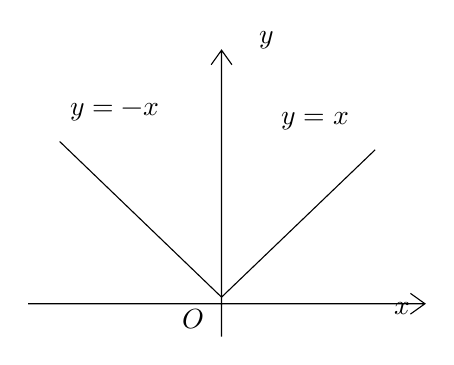
\begin{tikzpicture}[x=0.75pt,y=0.75pt,yscale=-1,xscale=1]
                              \draw  (95,215.74) -- (286.14,215.74)(188.14,93.57) -- (188.14,231.57) (279.14,210.74) -- (286.14,215.74) -- (279.14,220.74) (183.14,100.57) -- (188.14,93.57) -- (193.14,100.57)  ;
                              \draw    (110.14,137.57) -- (188.14,212.57) ;
                              \draw    (262.14,141.57) -- (188.14,212.57) ;
                              \draw (168,217) node [anchor=north west][inner sep=0.75pt]   [align=left] {$\displaystyle O$};
                              \draw (205,83) node [anchor=north west][inner sep=0.75pt]   [align=left] {$\displaystyle y$};
                              \draw (270,214) node [anchor=north west][inner sep=0.75pt]   [align=left] {$\displaystyle x$};
                              \draw (114,118) node [anchor=north west][inner sep=0.75pt]   [align=left] {$\displaystyle y=-x$};
                              \draw (216,122) node [anchor=north west][inner sep=0.75pt]   [align=left] {$\displaystyle y=x$};
                          \end{tikzpicture}
                      \end{center}
                  \end{solution}
            \item 研究$y=f\left(x\right)=x^{\frac13}$在$x=0$处的切线问题
                  \begin{solution}
                      显然,在$x=0$ 处$\dfrac{\Delta y}{\Delta x}=\dfrac{f(0+\Delta x)-f(0)}{\Delta x}=\dfrac{(\Delta x)^{\frac13}}{\Delta x}=\dfrac{1}{(\Delta x)^{\frac{2}{3}}}$
                      当$\Delta x>0$ 时,$f_{+}^{\prime}(0)=\lim_{\Delta x\to0^{+}}\dfrac{1}{\left(\Delta x\right)^{\frac{2}{3}}}=+\infty$
                      $\Delta x<0$ 时,$f_{-}^{\prime}(0)=\lim_{\Delta x\to0^{-}}\dfrac{1}{\left(\Delta x\right)^{\frac{2}{3}}}=+\infty$
                      这样的结果称为无穷导数.又$±\infty$被叫作广义的数,所以无穷导数在有些数学场合也可被视为导数存在的特殊情形.但是在考研中无穷被认为是不存在
                  \end{solution}
        \end{itemize}
    \end{criterion}
    \subsection{高阶导数}
    \begin{defn}{高阶导数的定义}{}
        函数$y=f(x)$具有$n$阶导数,也常说成函数$f(x)$为$n$阶可导,如果函数$f(x)$在点$x$处具有$n$阶导数,那么$f(x)$在点$x$的某一邻域内必定具有一切低于$n$阶的导数.二阶及二阶以上的导数统称为高阶导数.
        记作:
        $$
            f^{(n)}(x_0)=\lim_{\Delta x\to0}\dfrac{f^{(n-1)}(x_0+\Delta x)-f^{(n-1)}(x_0)}{\Delta x}\text{或}f^{(n)}(x_0)=\lim_{x\to x_0}\dfrac{f^{(n-1)}(x)-f^{(n-1)}(x_0)}{x-x_0}
        $$
        当$n=2$时:
        $$
            f^{\prime\prime}(x_0)=\lim_{\Delta x\to0}\dfrac{f^{\prime}(x_0+\Delta x)-f^{\prime}(x_0)}{\Delta x}\text{或}f^{\prime\prime}(x_0)=\lim_{x\to x_0}\dfrac{f^{\prime}(x)-f^{\prime}(x_0)}{x-x_0}
        $$
    \end{defn}
    \begin{corollary}{\textcolor{red}{$n$阶导数与$n-1$阶导数的关系}}{}
        如果$f(x)$在点$x_0$处有二阶导数,则$f(x)$在$x_0$的某个邻域内有一阶导数且$f^\prime(x)$在$x_0$处连续.\\
        如果$f(x)$在点$x_{0}$处有$n$阶导数,则$f(x)在x_0$的某个邻域内有$1 \sim (n-1)$阶连续的各阶导数.
    \end{corollary}
    \section{微分}
    \subsection{微分的概念}
    \begin{defn}{微分的定义}{}
        设函数$y=f(x)$在点 $x_0$的某邻域内有定义,且 $x_0+\Delta x$ 在该邻域内,对于函数增量
        $$\Delta y= f( x_0+ \Delta x) - f( x_0)$$
        若存在与$\Delta x$无关的常数$A$,使得$\Delta y=A\Delta x+o(\Delta x)$,其中$o(\Delta x)$是在 $\Delta x \to 0$ 时比 $\Delta x$更高阶的无穷小,则称$f(x)$在点 $x_0$处可微,并把增量的主要部分 $A\Delta x$ 称为\textbf{线性主部},也叫作\textbf{$f(x)$在点 $x_0$处的微分},记 \textcolor{red}{$dy|_x=x_0=A\Delta x$} 或 \textcolor{red}{$dy|_x=x_0=f^{\prime}(x_0)dx$}.
    \end{defn}
    \begin{problem}
    设 $f(x)$ 可导且 $f^\prime(x_0)=\dfrac12$,则当$\Delta x\to0$ 时$,f(x)$在$x_0$处的微分$\operatorname{dy}$是$\Delta x$的( )无穷小.\\
    A.等价 \quad B.同阶 \quad C.低阶 \quad D.高阶
    \end{problem}
    \begin{solution}
        因为$dy=f'(x) \Delta x=\dfrac{1}{2}\Delta x$,显然为同阶无穷小.
    \end{solution}
    \begin{problem}
    设函数$f(u)$可导,且$y=f(x^2)$,当自变量$x$在$x=-1$ 处取得增量 $\Delta x=-0.1$ 时,相应的函数增量 $\Delta y$ 的线性主部为 0.1,则$f^\prime(1)=$
    \end{problem}
    \begin{solution}
        $\mathrm{d}y=f'(x^2)\mathrm{d}(x^2)=2xf'(x^2)\mathrm{d}x=2xf'(x^2)\Delta x$,代入可得$f'(1)=0.5$
    \end{solution}
    \subsection{微分的几何意义}
    若$f(x)$在点$x_{0}$处可微,则在点$(x_0,y_0)$附近可以用切线段近似代替曲线段,这是可微的几何意义.
    \begin{center}
        \tikzset{every picture/.style={line width=0.75pt}} %set default line width to 0.75pt        
        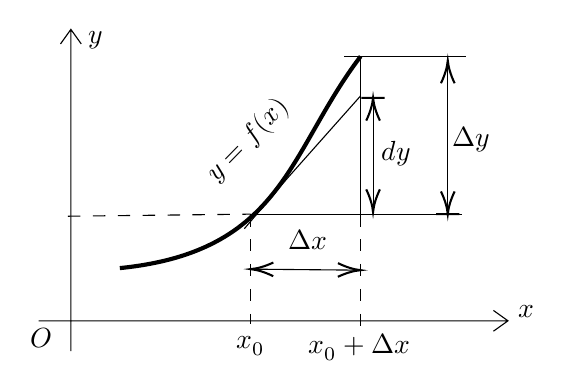
\begin{tikzpicture}[x=0.75pt,y=0.75pt,yscale=-1,xscale=1]
            \draw  (95,216.97) -- (321.14,216.97)(110.55,76.57) -- (110.55,231.57) (314.14,211.97) -- (321.14,216.97) -- (314.14,221.97) (105.55,83.57) -- (110.55,76.57) -- (115.55,83.57)  ;
            \draw [line width=1.5]    (250.14,89.57) .. controls (215.14,135.57) and (213.14,183.57) .. (134.14,191.57) ;
            \draw    (194.14,172.57) -- (214.88,148.26) -- (250.14,108.57) ;
            \draw  [dash pattern={on 4.5pt off 4.5pt}]  (109.14,166.57) -- (197.14,165.57) ;
            \draw  [dash pattern={on 4.5pt off 4.5pt}]  (197.14,165.57) -- (197.14,218.57) ;
            \draw    (197.14,165.57) -- (299.14,165.57) ;
            \draw    (250.14,108.57) -- (250.14,165.57) ;
            \draw  [dash pattern={on 4.5pt off 4.5pt}]  (250.14,165.57) -- (250.14,219.57) ;
            \draw    (242.14,89.57) -- (301.14,89.57) ;
            \draw    (292.14,93.57) -- (292.14,165.57) ;
            \draw [shift={(292.14,165.57)}, rotate = 270] [color={rgb, 255:red, 0; green, 0; blue, 0 }  ][line width=0.75]    (0,5.59) -- (0,-5.59)(10.93,-3.29) .. controls (6.95,-1.4) and (3.31,-0.3) .. (0,0) .. controls (3.31,0.3) and (6.95,1.4) .. (10.93,3.29)   ;
            \draw [shift={(292.14,91.57)}, rotate = 90] [color={rgb, 255:red, 0; green, 0; blue, 0 }  ][line width=0.75]    (10.93,-3.29) .. controls (6.95,-1.4) and (3.31,-0.3) .. (0,0) .. controls (3.31,0.3) and (6.95,1.4) .. (10.93,3.29)   ;
            \draw    (256.14,109.57) -- (256.14,162.57) ;
            \draw [shift={(256.14,164.57)}, rotate = 270] [color={rgb, 255:red, 0; green, 0; blue, 0 }  ][line width=0.75]    (10.93,-3.29) .. controls (6.95,-1.4) and (3.31,-0.3) .. (0,0) .. controls (3.31,0.3) and (6.95,1.4) .. (10.93,3.29)   ;
            \draw [shift={(256.14,109.57)}, rotate = 90] [color={rgb, 255:red, 0; green, 0; blue, 0 }  ][line width=0.75]    (0,5.59) -- (0,-5.59)(10.93,-3.29) .. controls (6.95,-1.4) and (3.31,-0.3) .. (0,0) .. controls (3.31,0.3) and (6.95,1.4) .. (10.93,3.29)   ;
            \draw    (250.14,89.57) -- (250.14,108.57) ;
            \draw    (248.14,192.55) -- (199.14,192.09) ;
            \draw [shift={(197.14,192.07)}, rotate = 0.54] [color={rgb, 255:red, 0; green, 0; blue, 0 }  ][line width=0.75]    (10.93,-3.29) .. controls (6.95,-1.4) and (3.31,-0.3) .. (0,0) .. controls (3.31,0.3) and (6.95,1.4) .. (10.93,3.29)   ;
            \draw [shift={(250.14,192.57)}, rotate = 180.54] [color={rgb, 255:red, 0; green, 0; blue, 0 }  ][line width=0.75]    (10.93,-3.29) .. controls (6.95,-1.4) and (3.31,-0.3) .. (0,0) .. controls (3.31,0.3) and (6.95,1.4) .. (10.93,3.29)   ;
            \draw (90,219) node [anchor=north west][inner sep=0.75pt]   [align=left] {$\displaystyle O$};
            \draw (118,76) node [anchor=north west][inner sep=0.75pt]   [align=left] {$\displaystyle y$};
            \draw (325,208) node [anchor=north west][inner sep=0.75pt]   [align=left] {$\displaystyle x$};
            \draw (171.74,143.51) node [anchor=north west][inner sep=0.75pt]  [rotate=-314.36] [align=left] {$\displaystyle y=f( x)$};
            \draw (293,122) node [anchor=north west][inner sep=0.75pt]   [align=left] {$\displaystyle \Delta y$};
            \draw (259,129) node [anchor=north west][inner sep=0.75pt]   [align=left] {$\displaystyle dy$};
            \draw (189,223) node [anchor=north west][inner sep=0.75pt]   [align=left] {$\displaystyle x_{0}$};
            \draw (224,222) node [anchor=north west][inner sep=0.75pt]   [align=left] {$\displaystyle x_{0} +\Delta x$};
            \draw (214,172) node [anchor=north west][inner sep=0.75pt]   [align=left] {$\displaystyle \Delta x$};
        \end{tikzpicture}
    \end{center}
    \section{导数的计算}
    \subsection{导数定义求导数}
    可以利用如下的公式进行导数定义求导数.
    $$
        f^{'}(x_{0})=\lim_{x\to x_{0}}\frac{f(x)-f(x_{0})}{x-x_{0}}=\lim_{\Delta x\to0}\frac{f(x_{0}+\Delta x)-f(x_{0})}{\Delta x}
    $$
    \begin{problem}
    设函数 $f(x)$ 在 $x=0$ 处可导,且 $f(0)=0$,则$\lim_{x\to0}\dfrac{x^2f(x)-2f(x^3)}{x^3}=$\\
    (A) $-2f'(0)$ \quad (B) $-f'(0)$ \quad (C) $f'(0)$ \quad (D)0
    \end{problem}
    \begin{solution}
        已知函数$f(x)$在$x=0$处可导,且$f(0)=0$,则$f(x)$在该$x=0$处一定连续,且$\lim_{x\to 0}\dfrac{f(x)}{x}=f'(0)$,则$\lim_{x\to0}\dfrac{x^2f(x)-2f(x^3)}{x^3}=\lim_{x\to 0}(\dfrac{f(x)}{x}-\dfrac{2f(x^3)}{x^3})=-f'(0)$
    \end{solution}
    \begin{note}
        看见函数在$0$点可导且$f(0)=0$,应想到$\lim_{x \to 0}\dfrac{f(x)}{x}=f'(0)$
    \end{note}
    \begin{problem}
    设曲线 $y=f(x)$ 与 $y=x^2-x$ 在点$(1,0)$ 处有公共切线,则$\lim_{n\to\infty}n f(\dfrac{n}{n+2})=$
    \end{problem}
    \begin{solution}
        已知$y=f(x)$与$y=x^2-x$在点$(1,0)$处有公共切线,则$f(1)=0,f'(1)=1$.则$\lim_{n \to \infty}\dfrac{f(\dfrac{n}{n+2})}{\dfrac{1}{n}}=\lim_{n \to \infty} \dfrac{f(1-\dfrac{2}{n+2})-f(1)}{\dfrac{1}{n}}=\lim_{n\to \infty}\dfrac{f(1-\dfrac{2}{n+2})-f(1)}{-\dfrac{2}{n+2}}\cdot \dfrac{-\dfrac{2}{2+n}}{\dfrac{1}{n}}=\lim_{n\to \infty} \dfrac{-2n}{2+n}=-2$
    \end{solution}
    \begin{note}
        此类题目应想办法结合题意构造导数定义式
    \end{note}
    \begin{problem}
    设函数$y=f(x)=
        \begin{cases}x & =2t+|t|,   \\
             y & =|t|\sin t
        \end{cases}$确定,则\\
    (A)$f(x)$ 连续$,f^\prime(0)$ 不存在. \quad (B)$f^\prime(0)$ 存在$,f^\prime(x)$ 在$x=0$ 处不连续. \\
    (C)$f^\prime(x)$ 连续,$f^{\prime\prime}(0)$ 不存在. \quad (D)$f^{\prime\prime}(0)$ 存在$,f^{\prime\prime}(x)$ 在$x=0$ 处不连续.
    \end{problem}
    \begin{solution}
        $x=\begin{cases}
                3t,t \geq 0 \\
                t,t<0
            \end{cases}$,联立$y=|t|\sin t$消去$t$可得$f(x)=\begin{cases}
                \dfrac{x}{3}\sin \dfrac{x}{3} ,x\geq 0 \\
                -x\sin x, x < 0
            \end{cases}$.
        $\lim_{x\to 0^-}=0=\lim_{x\to 0^+}$,又$f(0)=0$,又因为当$x\neq0$时函数显然连续,综上函数$f(x)$为连续函数.排除BD选项.$ f_+'(0)=\lim_{x\to 0^+} \dfrac{f(x)-f(0)}{x-0}=\lim_{x\to 0^+}\dfrac{\dfrac{x}{3}\sin\dfrac{x}{3}}{x}=0$,$f_{-}^{\prime}(0)=\lim_{x\to0^{-}}\dfrac{f(x)-f(0)}{x-0}=\lim_{x\to0^{-}}\dfrac{-x\sin x}{x}=0$.综上$f'(0)$存在.排除A选项.综上本题应该选择C选项.
    \end{solution}
    \begin{note}
        此题不能使用参数方程求导公式,因此只能将函数求出来.此外CD选项如果的后面的$f''(x)$的关系,应该使用二阶导数单侧的定义式来求解.
    \end{note}
    \begin{problem}
    设 $y=f(x)$ 由参数方程$\begin{cases}x=t^2+1,\\y=4t-t^2\end{cases}(t\geqslant0)$确定,则$\lim_{n\to\infty} n\left[f\left(\dfrac{2n+1}n\right)-3\right]=$
    \end{problem}
    \begin{solution}
        $\lim_{n \to \infty}\dfrac{f(\dfrac{2n+1}{n})-3}{\dfrac1n}=\lim_{n \to \infty}\dfrac{f(2+\dfrac{1}{n})-3}{\dfrac{1}{n}}$,如果$f(2)=3$,则上式值为$f'(2)$\\
        令$x=2$,代入参数方程可得$y=3$.使用参数方程求导公式可得$f'(2)=1$
    \end{solution}
    \subsection{基本求导公式}
    \begin{center}
        \boxed{
            $$
                \begin{aligned}
                     & \left(C\right)^{\prime}=0;                              &  & \left(x^{\alpha}\right)^{\prime}=\alpha x^{\alpha-1};      \\
                     & \left(a^{x}\right)^{\prime}=a^{x}\ln a;                 &  & \left(\mathrm{e}^{x}\right)^{\prime}=\mathrm{e}^{x};       \\
                     & \left(\log_{a}x\right)^{\prime}=\dfrac{1}{x\ln a};      &  & (\ln|x|)^{\prime}=\dfrac{1}{x};                            \\
                     & \left(\sin x\right)^{\prime}=\cos x;                    &  & \left(\cos x\right)^{\prime}=-\sin x;                      \\
                     & \left(\tan x\right)^{\prime}=\sec^{2}x;                 &  & \left(\cot x\right)^{\prime}=-\csc^{2}x;                   \\
                     & (\sec x)'=\sec x\tan x;                                 &  & (\csc x)'=-\csc x\cot x;                                   \\
                     & (\arcsin x)'=\dfrac{1}{\sqrt{1-x^2}};                   &  & (\arccos x)'=-\frac{1}{\sqrt{1-x^2}};                      \\
                     & (\arctan x)'=\dfrac{1}{1+x^2};                          &  & (\operatorname{arccot}x)'=-\frac{1}{1+x^2}.                \\
                     & [\ln(x+\sqrt{x^2+1})]^{\prime}=\dfrac{1}{\sqrt{x^2+1}}; &  & [\ln(x+\sqrt{x^{2}-1})]^{\prime}=\dfrac{1}{\sqrt{x^{2}-1}}
                \end{aligned}
            $$
        }
    \end{center}
    \subsection{导数运算法则}
    \subsubsection{导数运算四则运算}
    设$u=u(x),v=v(x)$在$x$处可导,则
    $$
        (u\pm v)^{\prime}=u^{\prime}\pm v^{\prime}
    $$
    $$
        \left(uv\right)^{\prime}=u^{\prime}v+uv^{\prime}
    $$
    $$
        \left(\dfrac uv\right)^{\prime}=\dfrac{u^{\prime}v-uv^{\prime}}{v^2}\quad(v\neq0)
    $$
    \subsubsection{复合函数导数运算法则}
    \begin{defn}{复合函数导数的定义}{}
        设$y = f ( g ( x ) )$是由$y=f(z)$,$z=g(x)$复合而成,且$f(z)$,$g(x)$均可导,则$\{f[g(x)]\}'=f'[g(x)]g'(x)$
    \end{defn}
    \subsection{分段函数的导数}
    设$f(x)=\begin{cases}f_1(x),&x\geqslant x_0,\\f_2(x),&x<x_{0},\end{cases}$其中$f_1(x),f_2(x)$分别在$x>x_0,x<x_0$时可导,则
    \begin{itemize}
        \item 在分段点$x_{\mathrm{o}}$处用导数定义求导$:f_+^{\prime}(x_0)=\lim_{x\to x_0^+}\dfrac{f_1(x)-f(x_0)}{x-x_0},f_-^{\prime}(x_0)=\lim_{x\to x_0^-}\dfrac{f_2(x)-f(x_0)}{x-x_0}$ .根据$f_+^{\prime}(x_0)$ 是否等于$f_-^{\prime}(x_0)$来判定$f^{\prime}(x_0);$
        \item 在非分段点用导数公式求导,即$x>x_0$时,$f^{\prime}(x)=f_1^{\prime}(x);x<x_0$时,$f^{\prime}(x)=f_2^{\prime}(x)$
    \end{itemize}
    \subsection{反函数的导数}
    \begin{defn}{反函数导数的定义}{}
        设$y=f(x)$为单调、可导函数,且$f^{\prime}(x)\neq0$,则存在反函数$x=\varphi(y)$,且$\dfrac{\mathrm{d}x}{\mathrm{d}y}=\dfrac{1}{\dfrac{dy}{dx}}$,即 $\varphi^{\prime}(y)=\dfrac1{f^{\prime}(x)}$
    \end{defn}
    \begin{defn}{反函数的二阶导数的定义}{}
        在$y=f(x)$单调,且二阶可导的情况下,若$f^{\prime}(x)\neq0$,则存在反函数$x=\varphi(y)$,记$f^{\prime}(x)=y_x^{\prime},\varphi^{\prime}\left(y\right)=x_{y}^{\prime}$,则有
        $$
            y_{x}^{\prime}=\dfrac{\mathrm{d}y}{\mathrm{d}x}=\dfrac{1}{\dfrac{\mathrm{d}x}{\mathrm{d}y}}=\frac{1}{x_{y}^{\prime}}
        $$
        $$
            y_{xx}^{\prime\prime}=\dfrac{\mathrm{d}^{2}y}{\mathrm{d}x^{2}}=\dfrac{\mathrm{d}\left(\dfrac{\mathrm{d}y}{\mathrm{d}x}\right)}{\mathrm{d}x}=\dfrac{\mathrm{d}\left(\dfrac{1}{x_{y}^{\prime}}\right)}{\mathrm{d}x}=\dfrac{\mathrm{d}\left(\dfrac{1}{x_{y}^{\prime}}\right)}{\mathrm{d}y}\cdot\dfrac{1}{x_{y}^{\prime}}=-\dfrac{1}{(x_{y}^{\prime})^{2}}\cdot(x_{y}^{\prime})_{y}^{\prime}\cdot\dfrac{1}{x_{y}^{\prime}}=-\dfrac{x_{yy}^{\prime\prime}}{(x_{y}^{\prime})^{2}}\cdot\dfrac{1}{x_{y}^{\prime}}=-\dfrac{x_{yy}^{\prime\prime}}{(x_{y}^{\prime})^{3}}
        $$
        反过来则有:
        $$
            x_{y}^{\prime}=\dfrac{1}{y_{x}^{\prime}},x_{yy}^{\prime\prime}=-\dfrac{y_{xx}^{\prime\prime}}{(y_{x}^{\prime})^{3}}
        $$\footnote{\textcolor{red}{此处非常容易错误的认为反函数的二阶导数是$\dfrac{1}{f''(x)}$}}
    \end{defn}
    \begin{problem}
    \getRating{1}设 $y=f(x)$ 的反函数是$x=\varphi(y)$,且 $f(x)=\int_1^{2x}\mathrm{e}^{t^2}\mathrm{d}t+1$,则 $\varphi^{\prime\prime}(1)=$
    \end{problem}
    \begin{solution}
        由反函数求导法得
        $$
            \varphi^{'}(y)=\frac{\mathrm{d}x}{\mathrm{d}y}=\dfrac{1}{\dfrac{\mathrm{d}y}{\mathrm{d}x}}=\frac{1}{f^{'}(x)}
        $$
        上式两端对$y$求导得
        $$
            \varphi''(y)=\frac{\mathrm{d}}{\mathrm{d}x}\biggl[\frac{1}{f'(x)}\biggr]\cdot\frac{\mathrm{d}x}{\mathrm{d}y}=-\frac{f''(x)}{\bigl[f'(x)\bigr]^2}\cdot\frac{1}{f'(x)}.
        $$
        由 $f(x)=\int_1^{2 x} \mathrm{e}^{t^2} \mathrm{~d} t+1$ 知, $x=\dfrac{1}{2}$ 时 $y=1$, 且
        $$
            f^{\prime}(x)=2 \mathrm{e}^{4 x^2}, f^{\prime \prime}(x)=16 x \mathrm{e}^{4 x^2}
        $$
        则 $\varphi^{\prime \prime}(1)=-\frac{f^{\prime \prime}\left(\dfrac{1}{2}\right)}{\left[f^{\prime}\left(\dfrac{1}{2}\right)\right]^3}=-\dfrac{8 \mathrm{e}}{8 \mathrm{e}^3}=-\dfrac{1}{\mathrm{e}^2}$.
    \end{solution}
    \begin{note}
        代入时一定要注意变量是自变量还是因变量,不可以带错.
    \end{note}
    \subsection{参数方程求导}
    \begin{defn}{参数方程所确定的函数的导数}{}
        设$y=f(x)$的参数方程是$\left\{\begin{aligned}x&=\varphi(t),\\y&=\psi (t),\end{aligned}\right.(\alpha<t<\beta)$确定的函数

        如果$\varphi(t)$和$\psi(t)$都可导,且$\varphi'(t) \neq 0$则其一阶导可写为
        $$
            \dfrac{\mathrm{d}y}{\mathrm{d}x}=\frac{\psi^{\prime}(t)}{\varphi^{\prime}(t)}
        $$
        若$\varphi(t)$ 和$\psi(t)$ 二阶可导,且 $\varphi^{\prime}(t)\neq 0$,则
        $$
            \begin{aligned}
                \frac{\operatorname{d}^2y}{\operatorname{d}x^2} & =\frac{d}{dx}(\frac{dy}{dx}) =\textcolor{red}{\frac{\operatorname{d}}{\operatorname{d}t}\Big(\frac{\psi'(t)}{\varphi'(t)}\Big) \times \frac{1}{\varphi'(t)}} \\
                                                                & =\frac{\psi''(t)\varphi'(t)-\varphi''(t)\psi'(t)}{\varphi'^2(t)}\times \frac{1}{\varphi'(t)}                                                                 \\
                                                                & =\frac{\psi''(t)\varphi'(t)-\varphi''(t)\psi'(t)}{\varphi'^3(t)}
            \end{aligned}
        $$
    \end{defn}
    \begin{problem}
    设 $y=y(x)$ 由$\begin{cases}x=3t^2+2t+3\\\mathrm{e}^y\sin t-y+1=0\end{cases}$确定,求$\dfrac{\mathrm{d}^2y}{\mathrm{d}x^2}\Bigg\vert_{t=0}.$
    \end{problem}
    \begin{solution}
        $$\left.\frac{\mathrm{d}^2 y}{\mathrm{~d} x^2}\right|_{t=0}=\frac{y^{\prime \prime}(0) x^{\prime}(0)-x^{\prime \prime}(0) y^{\prime}(0)}{x^{\prime 3}(0)}.$$
        由 $x=3 t^2+2 t+3$ 知 $x^{\prime}=6 t+2, x^{\prime \prime}=6$, 则 $x^{\prime}(0)=2, x^{\prime \prime}(0)=6$.由 $e^v \sin t-y+1=0$ 知 $y(0)=1$, 且
        $$
            \mathrm{e}^y y^{\prime} \sin t+\mathrm{e}^y \cos t-y^{\prime}=0
        $$
        $$
            \left(\mathrm{e}^y y^{\prime}\right) \cos t+\left(\mathrm{e}^y y^{\prime}\right)^{\prime} \sin t+\mathrm{e}^y y^{\prime} \cos t-\mathrm{e}^y \sin t-y^{\prime \prime}=0
        $$
        令 $t=0$, 得 $y^{\prime}(0)=\mathrm{e}, y^{\prime \prime}(0)=2 \mathrm{e}^2$. 于是 $\left.\dfrac{\mathrm{d}^2 y}{\mathrm{~d} x^2}\right|_{t=0}=\dfrac{2 \mathrm{e}^2-3 \mathrm{e}}{4}$.
    \end{solution}
    \begin{note}
        参数方程的二阶导,优先考虑套公式
    \end{note}
    \begin{problem}
    设 $f^{\prime\prime}(t)\neq0$,有$\begin{cases}x=f^{\prime}(t)\:\\y=tf^{\prime}(t)-f(t)\:,\end{cases}$求$\dfrac{\mathrm{d}^2y}{\mathrm{d}x^2}$
    \end{problem}
    \begin{solution}
        $\dfrac{\mathrm{d}y}{\mathrm{d}x}=\dfrac{y^{\prime}(t)}{x^{\prime}(t)}=\dfrac{f^{\prime}(t)+tf^{\prime\prime}(t)-f^{\prime}(t)}{f^{\prime\prime}(t)}=t ,\dfrac{\mathrm{d}^{2}y}{\mathrm{d}x^{2}}=\dfrac{\mathrm{d}}{\mathrm{d}x}(t)=\dfrac{\mathrm{d}}{\mathrm{d}t}(t) \dfrac{\mathrm{d}t}{\mathrm{d}x}=1\times\dfrac{1}{x^{\prime}(t)}=\dfrac{1}{f^{\prime\prime}(t)}.$
    \end{solution}
    \begin{note}
        由于公式法的使用会出现三阶导数,但是本题没有说明三阶导数是否存在因此不可以使用公式法进行求解.
    \end{note}
    \subsection{变上下限求导}
    \begin{problem}
    设 $y=f(x)$ 由方程 $x=\int_1^{y-x}\sin^2\left(\dfrac{\pi t}4\right)\mathrm{d}t$确定,则$\lim_{n\to\infty}n\bigg[f\bigg(\dfrac1n\bigg)-1\bigg]$
    \end{problem}
    \begin{solution}
        令方程 $x=\int_1^{y-x}\sin^2\left(\dfrac{\pi t}4\right)\mathrm{d}t$的上下限$y-x=1$,得$x=0,y=1$,即$f(0)=1$.
        $$\lim_{n\to \infty}\dfrac{f(\dfrac{1}{n})-1}{\dfrac{1}{n}}=\lim_{n\to \infty}\dfrac{f(\dfrac{1}{n})-f(0)}{\dfrac{1}{n}}=f'(0).$$
        对方程对$x$求导得,$1=(y'-1) \sin^2 [\dfrac{\pi}{4}(y-x)]$,代入$x=0,y=1$得$f'(0)=3.$
    \end{solution}
    \begin{note}
        看见变上下限积分,应想到令其上下限相等来得到特殊条件.
    \end{note}
    \begin{problem}
    设可导函数$y=y(x)$由方程$\sin x- \int _x^y\varphi ( u) du= 0$确定,其中可导函数$\varphi(u)>0$,且 $\varphi(0)=\varphi^\prime(0)=1$,求 $y^{\prime\prime}(0).$
    \end{problem}
    \begin{solution}
        令方程$\sin x- \int _x^y\varphi (u) du= 0$中的$\int_x^y \varphi(u)du $上下限相等得$x=y=0$.对方程两侧关于$x$求导得: $\cos x-[\varphi(y)y'-\varphi(x)]=0$.$x=0,y=0$代入$y(x)$得$y'(0)=2$.对$\cos x-[\varphi(y)y'-\varphi(x)]=0$.$x=0,y=0$两端对$x$求导得$-\sin x-\left[\varphi^{\prime}(y)y^{\prime2}+\varphi(y)y^{\prime\prime}-\varphi^{\prime}(x)\right]=0 $,代入可得$y''(0)=-3$.
    \end{solution}
    \subsection{隐函数求导}
    \subsubsection{隐函数的定义}
    \begin{defn}{隐函数与显函数的定义}{}
        \begin{itemize}
            \item 隐函数:$y$与$x$的关系隐含在一个等式中,$F(x,y)=0$,如$x^2+y^2=4$
            \item  显函数:因变量与自变量在等式两端,$y$和$x$各占一边,如$y=3x$​
        \end{itemize}
    \end{defn}
    \subsubsection{隐函数求导}
    \begin{defn}{隐函数求导法则}{}
        设函数$y=y(x)$是由方程$F(x,y)=0$ 确定的可导函数则
        \begin{itemize}
            \item 方程$F(x,y)=0$ 两边对自变量$x$求导,注意$y=y(x)$,即将$y$看作中间变量,得到一个关于$y^{\prime}$ 的方程
            \item 解该方程便可求出$y^{\prime}$
        \end{itemize}
    \end{defn}
    \begin{problem}
    设函数 $y=y(x)$ 由 $y-x\mathrm{e}^y=1$ 确定,试求$\dfrac{\mathrm{d}^2y}{\mathrm{d}x^2}\Bigg|_{x=0}$
    \end{problem}
    \begin{solution}
        对方程$y-x\mathrm{e}^y=1$对$x$求导得:$y' - e^y-xy'e^y=0$,再次求导得$y'' -y'e^y-y'e^{y}-x\left(y'e^{y}\right)'=0$,将$x=0$代入上述方程易知$x=0,y=1,y'(0)=e$,从而可以得到$y^{''}=2e^2$
    \end{solution}
    \begin{problem}
    设函数$y=y(x)$由$\begin{cases}x=\arctan t,\\2y-ty^2+\mathrm{e}^t=5\end{cases}$所确定,则$\dfrac{\mathrm{d}y}{\mathrm{d}x}=$
    \end{problem}
    \begin{solution}
        使用参数方程求导公式可得$2\dfrac{dy}{dt}-y^2-2ty\dfrac{dy}{dt}+e^t=0,\dfrac{dx}{dt}=\dfrac{1}{1+t^2}$,最终可得:$\dfrac{\mathrm{d}y}{\mathrm{d}x}=\dfrac{(y^{2}-\mathrm{e}^{t})(1+t^{2})}{2(1-ty)}$
    \end{solution}
    \begin{note}
        对参数方程中求导数时,以本题的$\dfrac{dy}{dt}$为例,应将$t$视为自变量,$y$视为因变量,然后根据隐函数求导发展进行求导.
    \end{note}
    \subsection{利用函数性质求导数}
    \subsubsection{对数函数求导法}
    对于\textbf{多项相乘、相除、开方、乘方}的式子,一般先取对数再求导 .设$y=f(x)(f(x)>0)$,则
    \begin{itemize}
        \item 等式两边取对数,得 $\ln y=\ln f(x)$
        \item 两边对自变量$x$求导(同样注意$y=f(x)$,即将$y$看作中间变量),得
              $$
                  \dfrac{1}{y}y'=\begin{bmatrix}\ln f(x)\end{bmatrix}'\Rightarrow y'=\frac{yf'(x)}{f(x)}\
              $$
    \end{itemize}
    \begin{problem}
    设函数$y=y(x)$由方程$x\mathrm{e}^{f(y)}=\mathrm{e}^y\ln2$确定,其中$f$具有二阶导数,且$f^{\prime}\neq1$,则$\dfrac{\mathrm{d}^2y}{\mathrm{d}x^2}=$
    \end{problem}
    \begin{solution}
        方程$x\mathrm{e}^{f(y)}=\mathrm{e}^{y}\ln2$两端取对数,得$\ln x+f(y)=y+\ln(\ln2).$两端关于$x$求导,得$\dfrac1x+f^{\prime}(y)\cdot y^{\prime}=y^{\prime}$,两端继续关于$x$求导,得$-\dfrac1{x^2}+f^{\prime\prime}(y)\cdot(y^{\prime})^2+f^{\prime}(y)\cdot y^{\prime\prime}=y^{\prime\prime}$,由此可得
        $y''=-\dfrac{[1-f^{\prime}(y)]^{2}-f^{\prime\prime}(y)}{x^{2}[1-f^{\prime}(y)]^{3}}$
    \end{solution}
    \begin{problem}
    设 $y=\sqrt[3]{\dfrac{\left(x+1\right)\left(x+2\right)}{x\left(1+x^{2}\right)}}$,求 $y^\prime$
    \end{problem}
    \begin{solution}
        \begin{align*}
            \ln |y|=              & = \dfrac{1}{3}[\ln| x+1 |+\ln| x+2 |-\ln| x |-\ln(1+x^{2})]                                                                 \\
            \dfrac{y^{\prime}}{y} & =\dfrac{1}{3}\left(\dfrac{1}{x+1}+\dfrac{1}{x+2}-\dfrac{1}{x}-\dfrac{2x}{1+x^{2}}\right)                                    \\
            y^{\prime}            & =\dfrac{1}{3}\sqrt[3]{\dfrac{(x+1)(x+2)}{x(1+x^{2})}}\Big(\dfrac{1}{x+1}+\frac{1}{x+2}-\frac{1}{x}-\frac{2x}{1+x^{2}}\Big).
        \end{align*}
    \end{solution}
    \subsubsection{幂指函数求导法}
    对于$u(x)^{v(x)}$函数,可采用$e^{v(x)\ln u(x)}$进行转换求导
    然后求导,得
    $$
        \left[u(x)^{\nu(x)}\right]^{\prime}=\left[\mathrm{e}^{\nu(x)\ln u(x)}\right]^{\prime}=u(x)^{\nu(x)}\left[\nu^{\prime}(x)\ln u(x)+\nu(x)\cdot\frac{u^{\prime}(x)}{u(x)}\right]
    $$
    \begin{problem}
    $y=(1+x^2)^{\sin x}$
    \end{problem}
    \begin{solution}
        \begin{align*}
            \text{原式} & = e^{\sin x\ln(1+x^2)}                                                                 \\
                      & = e^{\sin x\ln(1+x^2)} \times [ \cos x \cdot \ln(1+x^2)+\sin x\cdot \dfrac{2x}{1+x^2}] \\
                      & = (1+x^{2})^{\sin x}\cdot[\cos x\ln(1+x^{2})+\dfrac{2 x \sin x}{1+x^{2}}]
        \end{align*}
    \end{solution}
    \begin{problem}
    设函数 $f(x)=(\mathrm{e}^x-1)(\mathrm{e}^{2x}-2)\cdotp\cdotp\cdotp(\mathrm{e}^{nx}-n)$,其中 $n$ 为正整数,则 $f^{\prime}(0)=$
    \end{problem}
    \begin{solution}{\textbf{方法一:}}
        显然 $f(0)=0$,则由导数定义得
        \begin{align*}
            f'(0) & =\lim_{x\to0}\frac{f(x)}{x}=\lim_{x\to0}\frac{(\mathrm{e}^x-1)(\mathrm{e}^{2x}-2)\cdots(\mathrm{e}^{nx}-n)}{x} \\&=\lim_{x\to0}\frac{\mathrm{e}^x-1}{x}\lim_{x\to0}(\mathrm{e}^{2x}-2)\cdotp\cdotp\cdotp(\mathrm{e}^{nx}-n)\\&=(1-2)(1-3)\cdotp\cdotp\cdotp(1-n)=(-1)^{n-1}(n-1)!.
        \end{align*}
    \end{solution}
    \begin{solution}{\textbf{方法二:}}
        显然 $f(0)=0$,令$g(x)=(e^{2x}-2)\dots(e^{nx}-n)$,则$f(x)=(e^x-1)g(x)$,对$f(x)$求导得$f'(x)=e^xg(x)+(e^x-1)g'(x)$,则$f'(0)=g(0)=-2\cdot-3 \dots -n=(-1)^{n-1}(n-1)!$
    \end{solution}
    \begin{note}
        此类问题的特征是函数一边为0,一边不为0.方法一是利用导数求导公式进行计算,在使用导数定义时,一般在极限问题上会遇见等价无穷小或者拉格朗日中值定理.方法二是将两个函数分开,然后使用复合函数求导公式进行计算.遇见此类问题应采用法二把等于0的和不为0的单独拎出来进行计算.
    \end{note}
    \begin{problem}
    \getRating{1}设函数 $f(x)=\begin{bmatrix}\tan\left(\dfrac{\pi}{4}x\right)-1\end{bmatrix}\begin{bmatrix}\tan\left(\dfrac{\pi}{4}x^{2}\right)-2\end{bmatrix}\cdotp\cdotp\cdotp\cdotp\left[\tan\left(\dfrac{\pi}{4}x^{100}\right)-100\right]$,则 $f^\prime(1)$
    \end{problem}
    \begin{solution}
        令$g(x)=\begin{bmatrix}\tan\left(\dfrac{\pi}{4}x^{2}\right)-2\end{bmatrix}\cdotp\cdotp\cdotp\cdotp\left[\tan\left(\dfrac{\pi}{4}x^{100}\right)-100\right]$,则$f(x)=\begin{bmatrix}\tan(\dfrac{\pi}{4}x)-x\end{bmatrix}g(x)$.则 $f'(x)=\dfrac\pi4\mathrm{sec}^2\left(\dfrac{\pi x}4\right)g(x)+\begin{bmatrix}\tan(\dfrac{\pi}{4}x)-x\end{bmatrix}g'(x),f'(1)=\dfrac{\pi}{2}g(1) + 0 \cdot g(1) = -\dfrac{99!}{2}\pi$
    \end{solution}
    \begin{note}
        此题还可以使用导数的定义式进行计算.
        \begin{align*}
            \text{原式} & = \lim_{x\to1}\dfrac{f(x)-f(1)}{x-1}                           \\
                      & = \lim_{x\to1}\dfrac{[\tan(\dfrac{\pi}{4}x)-1]\cdot g(1)}{x-1} \\
                      & = \lim_{x \to 1}\dfrac{\dfrac{\pi}{2}(x-1)g(1)}{x-1}           \\
                      & = \dfrac{\pi}{2}(1-2)(1-3)\dots(1-100)                         \\
                      & = -\dfrac{99!}{2}\pi
        \end{align*}
    \end{note}
    \subsection{高阶导数求导}
    \subsubsection{归纳法和公式法求高阶导数}
    常用高阶导数:
    $$
        \boxed{ \begin{aligned}
                 & \left[\sin(ax+b)\right]^{(n)}=a^{n}\sin\left(ax+b+\frac{n\pi}{2}\right) &  & \left[\cos(ax+b)\right]^{(n)}=a^{n}\cos\left(ax+b+\frac{n\pi}{2}\right) \\
                 & \left[\ln(ax+b)\right]^{(n)}=(-1)^{n-1}a^{n}\frac{(n-1)!}{(ax+b)^{n}}   &  & \left(\frac{1}{ax+b}\right)^{(n)}=(-1)^{n}a^{n}\frac{n!}{(ax+b)^{n+1}}  \\
                 & \left(e^{ax+b}\right)^{(n)}=a^{n}e^{ax+b}                               &  &
            \end{aligned}}
    $$
    \begin{problem}
    设 $f(x)=\dfrac x{2x^2-7x+6}$,求 $f^{(n)}(x)$.
    \end{problem}
    \begin{solution}
        \begin{align*}
            \text{原式} & = \dfrac{x}{2x^2-7x+6}                                                       \\
                      & =   \dfrac{x}{(2x-3)(x-2)}                                                   \\
                      & = \dfrac{2}{x-2}-\dfrac{3}{2x-3}                                             \\
                      & = (\dfrac{2}{x-2})^n-(\dfrac{3}{2x-3})^n                                     \\
                      & = (-1)^{n}\cdot n![\dfrac{2}{(x-2)^{n+1}}-\dfrac{3\cdot2^{n}}{(2x-3)^{n+1}}]
        \end{align*}
    \end{solution}
    \begin{note}
        可使用待定系数法和一阶留数定理来确定有理分式的系数.
        % 一阶留数定理//TODO
    \end{note}
    \begin{problem}
    \getRating{1}已知函数 $f(x)=\dfrac{x^2}{1-x^2}$, 则 $f^{(n)}(x)=$
    \end{problem}
    \begin{solution}
        $f(x)=\dfrac{x^2+1-1}{1-x^2}=-1+\dfrac{1}{(1-x)(1+x)}=-1+\dfrac{1}{2(1-x)}+\dfrac{1}{2(1+x)}$.
        根据公式易知$f^n(x)=\dfrac{1}{2}\cdot(\dfrac{1}{1-x})^{(n)}+\dfrac{1}{2}\cdot(\dfrac{1}{1+x})^{(n)}=\dfrac{n!}{2}[\dfrac{1}{(1-x)^{n+1}}+\dfrac{(-1)^{n}}{(1+x)^{n+1}}]$
    \end{solution}
    \begin{note}
        分子分母最高次相同$\Longrightarrow$提常数.
    \end{note}
    \begin{problem}
    设 $y=\ln(1-2x)$,则$y^{(10)}=$
    \end{problem}
    \begin{solution}
        根据$\left[\ln(ax+b)\right]^{(n)}=(-1)^{n-1}a^{n}\dfrac{(n-1)!}{(ax+b)^{n}}$,代入$n=10,a=-2,b=1$可得:$\dfrac{-9!\cdot2^{10}}{(1-2x)^{10}}$
    \end{solution}
    \begin{problem}\getRating{1}
    设 $f(x)=\dfrac{x^{10}}{1-x}$,则 $f^{(10)}(x)=$
    \end{problem}
    \begin{solution}
        $f(x)=\dfrac{x^{10}-1+1}{1-x}=\dfrac{(x-1)\cdot(x^{9}+x^{8}+\cdots+x+1)}{1-x}+\dfrac{1}{1-x}$
        \newline
        显然$f(x)^{10}=(\dfrac{1}{1-x})^{10}$,即$\dfrac{10!}{(1-x)^{11}}$
    \end{solution}
    \begin{note}
        本题主要使用了一个公式$x^{n}-1=(x-1)(x^{n-1}+x^{n-2}+\cdots+x^{2}+x+1)$
    \end{note}
    \begin{problem}
    设 $f(x)=\mathrm{e}^x\sin x$,求 $f^{(n)}(x)$.
    \end{problem}
    \begin{solution}
        $f'(x)=\mathrm{e}^x\sin x+\mathrm{e}^x\cos x=\mathrm{e}^x(\sin x+\cos x)=\sqrt{2}\mathrm{e}^x\sin(x+\dfrac{\pi}{4})$
        \newline
        $f''(x)=\sqrt{2} \sqrt{2} e^x \cdot \sin(x+\dfrac{\pi}{4}+\dfrac{\pi}{4})$
        \newline
        $f^{n}(x)=(\sqrt{2})^n\cdot e^x \cdot \sin(x+\dfrac{n\pi}{4})$
    \end{solution}
    \begin{note}
        本题为非常规形式的$n$阶导数,应当先试着求一次导来找规律.
    \end{note}
    \begin{problem}
    \getRating{1}设 $f(x)=\sin^4x+\cos^4x$,求 $f^{(n)}(x)$.
    \end{problem}
    \begin{solution}
        $f'(x)=-\sin 4x$,根据公式$\left[\sin(ax+b)\right]^{(n)}=a^{n}\sin\left(ax+b+\dfrac{n\pi}{2}\right)$
        \newline
        $f^{(n)}(x)=-4^{n-1} \cdot \sin(4x+\dfrac{n-1}{2}\pi)$
    \end{solution}
    \subsubsection{莱布尼兹公式求高阶导数}
    设$u=u(x),\nu=\nu(x)$均$n$阶可导,则
    $$
        (u\pm v)^{(n)}=u^{(n)}\pm v^{(n)}
    $$
    $$
        (u\nu)^{(n)}=u^{(n)}\nu+C_{n}^{1}u^{(n-1)}\nu^{\prime}+C_{n}^{2}u^{(n-2)}\nu^{\prime\prime}+\cdots+C_{n}^{k}u^{(n-k)}\nu^{(k)}+\cdots+C_{n}^{n-1}u^{\prime}\nu^{(n-1)}+u\nu^{(n)}=\sum_{k=0}^{n}C_{n}^{k}u^{(n-k)}\nu^{(k)}
    $$
    \subsubsection{泰勒公式求高阶导数}
    已知带佩亚诺余项的$n$阶泰勒展开式的条件为,如果函数$f(x)$在$x_0$处具有$n$阶导数,那么该函数的抽象展开为
    $$
        y=f(x)=\sum_{n=0}^{\infty}\dfrac{f^{(n)}(x_0)}{n!}(x-x_0)^n
    $$
    具体展开为:
    $$
        f(x)=f(x_{0})+f'(x_{0})(x-x_{0})+\dfrac{f''(x_{0})}{2!}(x-x_{0})^{2}+\cdots+\dfrac{f^{(n)}(x_{0})}{n!}(x-x_{0})^{n}+o\left(\left(x-x_{0}\right)^{n}\right)
    $$
    当$x_0=0$时
    $$
        y=f(x)=\sum_{n=0}^\infty\dfrac{f^{(n)}(0)}{n!}x^n
    $$
    具体展开为:
    $$
        f(x)=f(0)+f'(0)x+\cdots+\dfrac{f^{(n)}(0)}{n!}x^{n}+o(x^{n})
    $$
    函数泰勒展开式的唯一性:无论$f(x)$由何种方法展开,其泰勒展开式具有唯一性,那么就可以\textcolor{red}{通过与抽象展开和具体展开的系数的对比},获得$f^{(n)}(x_0)$或者$f^{(n)}(0)$
    \begin{center}
        \boxed{
            $$
                \begin{aligned}
                     & \dfrac{1}{1-x}=1+x+x^{2}+\cdots+x^{n}+\cdots=\sum_{n=0}^{\infty}x^{n}                                                           & (-1<x<1)            \\
                     & \dfrac{1}{1+x}=1-x+x^{2}-\cdots+(-1)^{n}x^{n}+\cdots=\sum_{n=0}^{\infty}(-1)^{n}x^{n}                                           & (-1<x<1)            \\
                     & \mathrm{e}^{x}=1+x+\dfrac{x^{2}}{2!}+\cdots+\dfrac{x^{n}}{n!}+\cdots=\sum_{n=0}^{\infty}\dfrac{x^{n}}{n!}                       & (-\infty<x<+\infty) \\
                     & \sin x=x-\dfrac{x^{3}}{3!}+\cdots+\dfrac{(-1)^{n}x^{2n+1}}{(2n+1)!}+\cdots=\sum_{n=0}^{\infty}\dfrac{(-1)^{n}x^{2n+1}}{(2n+1)!} & (-\infty<x<+\infty) \\
                     & \cos x=1-\frac{x^{2}}{2!}+\cdots+\frac{(-1)^{n}x^{2n}}{(2n)!}+\cdots=\sum_{n=0}^{\infty}\frac{(-1)^{n}x^{2n}}{(2n)!}            & (-\infty<x<+\infty) \\
                     & \ln(1+x)=x-\frac{x^{2}}{2}+\cdots+\frac{(-1)^{n-1}x^{n}}{n}+\cdots=\sum_{n=1}^{\infty}\frac{(-1)^{n-1}x^{n}}{n}                 & (-1<x\leqslant1)    \\
                     & (1+x)^{\alpha}= 1+ax+\frac{\alpha(\alpha-1)}{2!}x^{2}+\cdots+\frac{\alpha(\alpha-1)\cdots(\alpha-n+1)}{n!}x^{n}+\cdots                                \\
                     & = \sum_{n=0}^{\infty}\frac{\alpha(\alpha-1)\cdots(\alpha-n+1)}{n!}x^{n}                                                         & (-1<x<1)
                \end{aligned}
            $$
        }
    \end{center}
    \begin{problem}
    \getRating{1}求函数 $f(x)=x^2\ln(1+x)$ 在 $x=0$ 处的 $n(n>2)$ 阶导数.
    \end{problem}
    \begin{solution}{莱布尼兹公式:}
        \begin{align*}
            f^{(n)}(x) & = x^{2}\cdot[\ln(1+x)]^{(n)}+C_{n}^{1}\cdot2x\cdot[\ln(1+x)]^{(n-1)}+C_{n}^{2}\cdot2\cdot[\ln(1+x)]^{(n-2)} \\
            f^{(n)}(0) & =  C_{n}^{2}\cdot2\cdot[\ln(1+x)]^{(n-2)} |_{x=0}                                                           \\
                       & =  \dfrac{(-1)^{n-1}n!}{n-2}
        \end{align*}
    \end{solution}
    \begin{solution}{泰勒公式:}
        \begin{align*}
            f(x)       & = x^{2}\cdot(x-\frac{x^{2}}{2}+\ldots+\frac{(-1)^{n-3}\cdot x^{n-2}}{n-2}+\ldots) \\
            f(x)       & =   x^{3}-\frac{x^{4}}{2}+\cdots+(-1)^{n-1}\cdot\frac{x^{n}}{n-2}+\cdots          \\
            f^{(n)}(x) & =(-1)^{n-1}\frac{n!}{n-2}+x\cdot \square+x^{2}\cdot \square                       \\
            f^{(n)}(0) & =(-1)^{n-1}\cdot\dfrac{n!}{n-2}
        \end{align*}
    \end{solution}
    \section{导数的几何应用}
    \subsection{单调性判别}
    设函数$y=f(x)$在$[a,b]$上连续,在$(a,b)$内可导.
    \begin{itemize}
        \item 如果在(a,b)内$f^{\prime}(x)\geqslant0$,且等号仅在有限个点处成立,那么函数$y=f(x)$在$[a,b]$上严格单调增加
        \item 如果在(a,b)内$f^{\prime}(x)\leqslant0$,且等号仅在有限个点处成立,那么函数$y=f(x)$在$[a,b]$上严格单调减少
    \end{itemize}
    关于单调性的问题在第一章函数部分\ref{ddx}有更加详细的解释.
    \subsection{极值}
    \subsubsection{极值的定义}
    \begin{defn}{极值的定义}{}
        对于函数$f(x)$,若存在点$x_0$的某个邻域,使得在该邻域内任意一点$x$,均有
        $$
            f(x)\leqslant f(x_0)(\text{或}f(x)\geqslant f(x_0))
        $$
        成立,则称点$x_0$为$f(x)$的极大值点(或极小值点),$f(x_0)$为$f(x)$的极大值(或极小值).
    \end{defn}
    \begin{criterion}{极值的注意事项}{}
        \begin{itemize}
            \item 当题目询问极值点时,应写为$x=x_0$,其中$x_0$为极值点
            \item 端点出不讨论极值,因为单侧可能不存在
            \item 常函数某任一邻域内处处都是极值点
            \item 间断点也可以极值点,只要满足其邻域内最大值即可
            \item 极值点只能有两种情况,即驻点和不可导点:
                  \begin{enumerate}
                      \item 驻点:$f^{\prime}(x_{0})=0$,如$y=x^{2}$在$(0,0)$处的情形
                      \item 不可导点:$f^{\prime}(x_{0})$不存在,如$y=\left|x\right|$在$(0,0)$处的情形
                  \end{enumerate}
        \end{itemize}
    \end{criterion}
    \subsubsection{极值的判定}
    \begin{defn}{极值判定的必要条件}{}
        设$f(x)$在$x=x_0$处可导,且在点$x_0$处取得极值,则必有$f^{\prime}(x_0)=0$
    \end{defn}
    此外,通常把导数为零的点称为函数的驻点.
    \begin{defn}{极值判定的第一充分条件}{}
        设$f(x)$在$x=x_0$处连续,且在$x_0$的某去心邻域$\mathring U(x_0,\delta)(\delta>0)$内可导.
        \begin{enumerate}
            \item 若$x\in(x_0-\delta,x_0)$时$,f^\prime(x)<0$,而$x\in(x_0,x_0+\delta)$时$,f^\prime(x)>0$,则$f(x)$在$x=x_0$处取得极小值
            \item 若$x\in(x_0-\delta,x_0)$时$,f^\prime(x)>0$,而$x\in(x_0,x_0+\delta)$时$,f^\prime(x)<0$,则$f(x)$在$x=x_0$处取得极大值
            \item 若$f^\prime(x)$在$(x_0-\delta,x_0)$和$(x_0,x_0+\delta)$内不变号,则点$x_0$不是极值点
        \end{enumerate}
    \end{defn}
    简单概要第一充分条件,即:若$f(x)$在某点去心邻域内可导,则极值点\footnote{该点可以不可导,但是必须有定义,如$f(x)=|x|$}为去心邻域内导数变号的点.
    \begin{defn}{极值判定的第二充分条件}{}
        设$f(x)$在$x=x_0$处二阶可导,且$f^\prime(x_{0})=0,f^{\prime\prime}(x_{0})\neq0$
        \begin{enumerate}
            \item 若$f^{\prime\prime}(x_{0})<0,则f(x)$在$x_0$处取得极大值
            \item 若$f^{\prime\prime}(x_{0})>0,则f(x)$在$x_{0}$处取得极小值.
        \end{enumerate}
        \begin{proof}[极值判定的第二充分条件证明:]
            \begin{align*}
                f^{\prime\prime} (x_0) & =  \lim_{x\to x_0} \dfrac{f'(x)-f'(x_0)}{x-x_0} \\
                                       & = \lim_{x\to x_0} \dfrac{f'(x)}{x-x_0}
            \end{align*}
            若$x-x_0>0$且$f^{\prime\prime} (x_0)<0$,则$f'(x)<0$.若$x-x_0<0$且$f^{\prime\prime} (x_0)<0$,则$f'(x)>0$,那么$x_0$为极小值点.同理可得极大值点.
        \end{proof}
    \end{defn}
    第二充分条件的理解可以使用如下图像:
    \begin{center}
        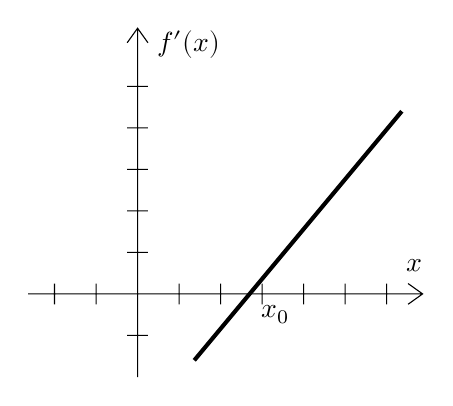
\begin{tikzpicture}[x=0.75pt,y=0.75pt,yscale=-1,xscale=1]
            \draw  (190,208) -- (380,208)(242.68,80) -- (242.68,248.15) (373,203) -- (380,208) -- (373,213) (237.68,87) -- (242.68,80) -- (247.68,87) (262.68,203) -- (262.68,213)(282.68,203) -- (282.68,213)(302.68,203) -- (302.68,213)(322.68,203) -- (322.68,213)(342.68,203) -- (342.68,213)(362.68,203) -- (362.68,213)(222.68,203) -- (222.68,213)(202.68,203) -- (202.68,213)(237.68,188) -- (247.68,188)(237.68,168) -- (247.68,168)(237.68,148) -- (247.68,148)(237.68,128) -- (247.68,128)(237.68,108) -- (247.68,108)(237.68,228) -- (247.68,228) ;
            \draw   ;
            \draw [color={rgb, 255:red, 0; green, 0; blue, 0 }  ,draw opacity=1 ][line width=1.5]    (270,240) -- (370,120) ;
            \draw (371.18,189.89) node [anchor=north west][inner sep=0.75pt]  [rotate=-0.51] [align=right] {$\displaystyle x$};
            \draw (301,212) node [anchor=north west][inner sep=0.75pt]   [align=left] {$\displaystyle x_{0}$};
            \draw (251,80) node [anchor=north west][inner sep=0.75pt]   [align=left] {$\displaystyle f'(x)$};
        \end{tikzpicture}
    \end{center}
    可以观察到$f'(x_0)=0$,当$f'(x)$在$x_0$邻域内存在不为0的点,导致该点为一个极值点.\textbf{此外应该首先考虑第二充分条件.}
    \begin{defn}{极值判定的第三充分条件}{}
        设$f(x)$在$x=x_0$处$n$ 阶可导,且$f^{(m)}(x_0)=0(m=1,2,\cdots,n-1),f^{(n)}(x_0)\neq0(n\geqslant2)$,则
        \begin{enumerate}
            \item 当$n$为偶数且$f^{(n)}(x_0)<0$时,$f(x)$在$x_0$处取得极大值
            \item 当$n$为偶数且$f^{(n)}(x_0)>0$ 时,$f(x)$在 $x_0$处取得极小值
        \end{enumerate}
    \end{defn}
    \begin{problem}
    设函数$f(x)$可导,且$f(x)f^\prime(x)>0$,则\\
    $(A)f(1)>f(-1)$ \quad $(B)f(1)<f(-1)$ \quad $(C)\left|f(1)\right|>\left|f(-1)\right|$ \quad $(D)\left|f(1)\right|<\left|f(-1)\right|$
    \end{problem}
    \begin{solution}
        $(\dfrac{1}{2}f^2(x))'=f(x)f'(x)>0$,那么$\dfrac{1}{2}f^2(x)$单增,对其开方可得:$|f(x)|$单增,随即得到$|f(1)|>|f(-1)|$,综上本题应当选择C选项.
    \end{solution}
    \begin{note}
        本题的难点在于构造函数$\dfrac{1}{2}f^2(x)$
    \end{note}
    \begin{problem}
    设函数$f(x)$二阶可导,且在$x=x_0$处取极大值,则有\\
    $(A)f^{\prime\prime}(x_0)<0$ \quad $(B)f^{\prime\prime}(x_0)\leqslant0$ \quad $(C)f^{\prime\prime}(x_0)>0$ \quad $(D)f^\prime\prime(x_0)\geqslant0$
    \end{problem}
    \begin{solution}
        取$f(x)=-x^4$,可知$f(x)$在$x=0$处取极大值,此时$f^{\prime\prime}(0)=0$.此外根据极值存在的第二充分条件,可以得到$f''(0)>0$,综上应当选择D选项.
    \end{solution}
    \begin{note}
        本题的易错点在于根据极值判定的第二充分条件,错误的认为了$f''(x)>0$,而忽略了这个仅是充分条件,不是必要条件.
    \end{note}
    \begin{problem}
    \getRating{1}设$f(x)$二阶可导,且$\operatorname*{lim}_{h\to0}\dfrac{f(x_{0}+h)-f(x_{0})-f^{\prime}(x_{0})}{h^{2}}=a\neq0$,试讨论$f(x)$在$x_{0}$点的极值.
    \end{problem}
    \begin{solution}
        由题目可知$\operatorname*{lim}_{h\to0}\dfrac{f(x_{0}+h)-f(x_{0})-f^{\prime}(x_{0})}{h^{2}}=a\neq0$,如果最终的极限不为0,那么说明分子的极限趋近于0,已知$f(x)$二阶可导,那么$f'(x_0)=0$.对$x_0$点进行求二阶导,可以判断出该点的极值.
        \begin{align*}
            \text{原式} & = \lim_{h\to 0}\dfrac{f(x_0+h)-f(x_0)}{h^2}  \\
                      & = \lim_{h\to 0}\dfrac{f'(x_0+h)-f'(x_0)}{2h} \\
                      & = \dfrac{1}{2}f^{''}(x_0)=a
        \end{align*}
        综上,当 $a>0$时,$x_0$为极小值点;当 $a<0$时,$x_0$为极大值点.
    \end{solution}
    \begin{problem}
    设函数$y=f(x)$由方程$y^{3}+xy^{2}+x^{2}y+6=0$确定,求$f(x)$的极值
    \end{problem}
    \begin{solution}
        对方程左右求导可得:$3y'y^2+y^2+2xyy'+x^2y'+2xy=0$.令$y'=0$得$y^2+2xy=0$,此时$y=0/-2x$.将$y=-2x$代入原方程可得$x=1,f(1)=-2,f'(1)=0$.对方程$3y'y^2+y^2+2xyy'+x^2y'+2xy=0$中变量$x$求导得:$6yy'^2+3y^2y''+4yy'+2xy'^2+2xyy''+2y+4xy'+x^2y''=0$.将$x=1,f(1)=-2,f'(1)=0$代入可得$f''(1)=\dfrac{4}{9}>0$.综上,函数$f(x)$在$x=1$处存在极小值,且$f(1)=-2$.
    \end{solution}
    \begin{problem}
    设 $y=f(x)$在$x_{0}$的某邻域内有四阶连续导数,且$f^{\prime}(x_{0})=f^{\prime\prime}(x_{0})=f^{\prime\prime\prime}(x_{0})=0$,且$f^{(4)}\left(x_{0}\right)<0$,则()\\
    A.$f(x)$在$x_{0}$处取得极小值\quad
    B.$f(x)$在$x_{0}$处取得极大值\\
    C.$(x_{0},f(x_{0}))$是$y=f(x)$的拐点\quad
    D.$f(x)$在$x_{0}$的某邻域内单调减少
    \end{problem}
    \begin{solution}
        根据第三充分条件,$n$为偶数时,且$f^4(x_0)<0$,则该点为极大值点.综上,应当选择B选项
    \end{solution}
    \begin{problem}
    \getRating{1}设$f(x)$在$x=0$的某邻域内连续,$f(0)=0,\operatorname*{lim}_{x\to0}\dfrac{f(x)}{1-\operatorname{cos}\,x}=2$,则$f(x)$在$x=0$处().\\
    A.不可导\quad B.可导且$f'(0)\neq0$\quad C.有极小值\quad D.有极大值
    \end{problem}
    \begin{solution}
        $\lim_{x\to 0} \dfrac{f(x)}{1-\cos x}=\lim_{x\to 0} \dfrac{f(x)}{\frac{1}{2}x^2}=2  \Rightarrow \lim_{x\to 0} \dfrac{f(x)}{x^2}=1$,则$\lim_{x\to 0}f(x)>0$,又因为$f(x)$在$x=0$连续,则$f(0)=0$,则$f(x)$在$x=0$时存在极小值.综上,应当选择C选项.
    \end{solution}
    \begin{problem}
    \getRating{1}设$f(x)$在$x_{0}$的某邻域内连续,且$\operatorname*{lim}_{x\to x_{0}}\dfrac{f(x)-f(x_{0})}{(x-x_{0})^{n}}=1$,则()\\
    A.当$n$为奇数时,$x_{0}$是$f(x)$的极大值点\quad
    B.当$n$为奇数时,$x_{0}$是$f(x)$的极小值点\\
    C.当$n$为偶数时$,x_{0}$是$f(x)$的极小值点\quad
    D.当$n$为偶数时,$x_{0}$是$f(x)$的极大值点
    \end{problem}
    \begin{solution}
        AB选项:令$n=1$可得,$f'(x_0)=1$,不存在极值点. CD选项:令$n=0$,则$\lim_{x\to x_0}f(x)-f(x_0)=1$,不符合题意.因此应当使$n=2$,则$\lim_{x\to x_0}f(x)-f(x_0)>0$,则$f(x_0)$为极小值点.综上,应当选择C选项.
    \end{solution}
    \subsection{最值}
    \begin{defn}{最值的定义}{}
        设$x_0$为$f(x)$定义域内一点,若对于$f(x)$的定义域内任意一点$x$,均有
        $$
            f(x)\leqslant f(x_0)(\text{或}f(x)\geqslant f(x_0))
        $$
        成立,则称$f(x_0$)为$f(x)$的最大值(或最小值).
    \end{defn}
    \begin{conclusion}{有关极值点和最值点的结论}{}
        \begin{enumerate}
            \item 若函数在闭区间$[a,b]$上的最大值(或最小值)在开区间$(a,b)$上某点取得,那么,函数在该点处必取得极大值(或极小值).
            \item $f(x)$在$(a,b)$上连续,若$f(x)$在$(a,b)$上有唯一极值点,则该点一定也是$(a,b)$上点最值点,但不一定是$[a,b]$上点最值点,因为可能存在跳跃间断点,如下图所示
                  \begin{center}
                      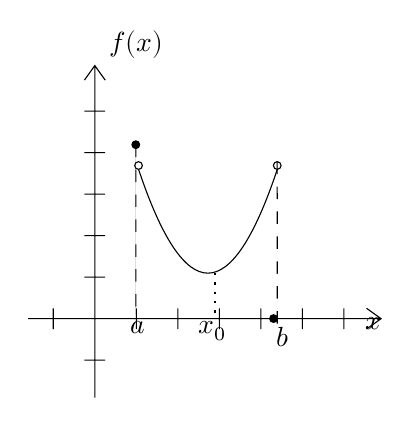
\begin{tikzpicture}[x=0.75pt,y=0.75pt,yscale=-1,xscale=1]
                          \draw  (70,201.93) -- (240,201.93)(102.08,80) -- (102.08,240) (233,196.93) -- (240,201.93) -- (233,206.93) (97.08,87) -- (102.08,80) -- (107.08,87) (122.08,196.93) -- (122.08,206.93)(142.08,196.93) -- (142.08,206.93)(162.08,196.93) -- (162.08,206.93)(182.08,196.93) -- (182.08,206.93)(202.08,196.93) -- (202.08,206.93)(222.08,196.93) -- (222.08,206.93)(82.08,196.93) -- (82.08,206.93)(97.08,181.93) -- (107.08,181.93)(97.08,161.93) -- (107.08,161.93)(97.08,141.93) -- (107.08,141.93)(97.08,121.93) -- (107.08,121.93)(97.08,101.93) -- (107.08,101.93)(97.08,221.93) -- (107.08,221.93) ;
                          \draw   ;
                          \draw   (123.17,130) .. controls (145.45,196.67) and (167.72,196.67) .. (190,130) ;
                          \draw  [dash pattern={on 0.84pt off 2.51pt}]  (160,180) -- (160,200) ;
                          \draw   (189.94,126.29) .. controls (188.92,126.31) and (188.1,127.15) .. (188.12,128.17) .. controls (188.13,129.2) and (188.98,130.02) .. (190,130) .. controls (191.02,129.98) and (191.84,129.14) .. (191.83,128.12) .. controls (191.81,127.09) and (190.97,126.27) .. (189.94,126.29) -- cycle ;
                          \draw   (123.12,126.29) .. controls (122.09,126.31) and (121.27,127.15) .. (121.29,128.17) .. controls (121.31,129.2) and (122.15,130.02) .. (123.17,130) .. controls (124.2,129.98) and (125.02,129.14) .. (125,128.12) .. controls (124.98,127.09) and (124.14,126.27) .. (123.12,126.29) -- cycle ;
                          \draw  [color={rgb, 255:red, 0; green, 0; blue, 0 }  ,draw opacity=1 ][fill={rgb, 255:red, 0; green, 0; blue, 0 }  ,fill opacity=1 ] (121.8,116.26) .. controls (120.77,116.28) and (119.95,117.12) .. (119.97,118.14) .. controls (119.99,119.17) and (120.83,119.99) .. (121.86,119.97) .. controls (122.88,119.95) and (123.7,119.11) .. (123.68,118.09) .. controls (123.66,117.06) and (122.82,116.24) .. (121.8,116.26) -- cycle ;
                          \draw  [fill={rgb, 255:red, 0; green, 0; blue, 0 }  ,fill opacity=1 ] (188.14,200.03) .. controls (187.12,200.05) and (186.3,200.89) .. (186.32,201.91) .. controls (186.34,202.94) and (187.18,203.76) .. (188.2,203.74) .. controls (189.23,203.72) and (190.05,202.88) .. (190.03,201.86) .. controls (190.01,200.83) and (189.17,200.01) .. (188.14,200.03) -- cycle ;
                          \draw  [dash pattern={on 4.5pt off 4.5pt}]  (189.94,126.29) -- (190,210) ;
                          \draw [fill={rgb, 255:red, 0; green, 0; blue, 0 }  ,fill opacity=1 ] [dash pattern={on 4.5pt off 4.5pt}]  (121.83,118.12) -- (121.86,199.97) ;
                          \draw (231.18,199.89) node [anchor=north west][inner sep=0.75pt]  [rotate=-0.51] [align=left] {$\displaystyle x$};
                          \draw (151,202) node [anchor=north west][inner sep=0.75pt]   [align=left] {$\displaystyle x_{0}$};
                          \draw (108,62) node [anchor=north west][inner sep=0.75pt]   [align=left] {$\displaystyle f( x)$};
                          \draw (118,202) node [anchor=north west][inner sep=0.75pt]   [align=left] {$\displaystyle a$};
                          \draw (188.32,204.91) node [anchor=north west][inner sep=0.75pt]   [align=left] {$\displaystyle b$};
                      \end{tikzpicture}
                  \end{center}
                  显然,从图中可以得到,在区间$(a,b)$,点$x_0$为极值点,但是在区间$[a,b]$上,并不是最值点.\\  但是如果增加条件$f(x)$在$[a,b]$上连续\footnote{即排除了跳跃间断点的情况},则$f(x)$在$(a,b)$上的唯一极值点也是$[a,b]$上点最值点.
        \end{enumerate}
    \end{conclusion}
    \subsection{凹凸性}
    \subsubsection{凹凸性的定义}
    \begin{defn}{凹凸性第一种的定义}{}
        设函数$f(x)$在区间$I$ 上连续.如果对 $I$ 上任意不同两点$x_1,x_2$,恒有
        $$
            f\left(\frac{x_{1}+x_{2}}{2}\right)<\dfrac{f(x_{1})+f(x_{2})}{2}
        $$
        则称 $y=f(x)$在$I$ 上的图形是凹的(或凹弧),即如下图所示
        \begin{center}
            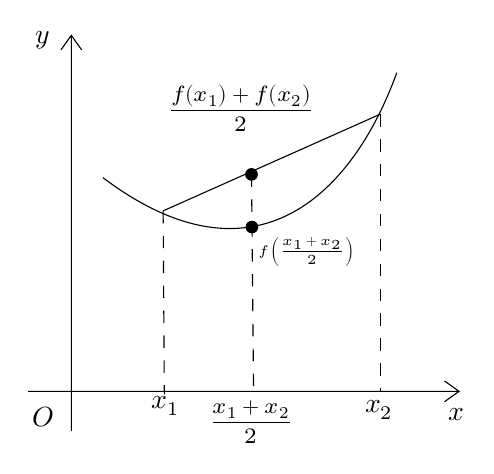
\begin{tikzpicture}[x=0.75pt,y=0.75pt,yscale=-1,xscale=1]
                \draw  (54,203.94) -- (261.57,203.94)(74.76,32.43) -- (74.76,223) (254.57,198.94) -- (261.57,203.94) -- (254.57,208.94) (69.76,39.43) -- (74.76,32.43) -- (79.76,39.43)  ;
                \draw    (90,101) .. controls (163.57,156.43) and (210.57,108.43) .. (231.57,50.43) ;
                \draw    (119,117) -- (223.57,70.43) ;
                \draw  [dash pattern={on 4.5pt off 4.5pt}]  (119,117) -- (119.57,205.43) ;
                \draw  [dash pattern={on 4.5pt off 4.5pt}]  (223.57,70.43) -- (223.57,204.43) ;
                \draw  [dash pattern={on 4.5pt off 4.5pt}]  (161.57,99.43) -- (162.57,203.43) ;
                \draw  [color={rgb, 255:red, 0; green, 0; blue, 0 }  ,draw opacity=1 ][fill={rgb, 255:red, 0; green, 0; blue, 0 }  ,fill opacity=1 ] (158.79,99.43) .. controls (158.79,97.89) and (160.03,96.64) .. (161.57,96.64) .. controls (163.11,96.64) and (164.36,97.89) .. (164.36,99.43) .. controls (164.36,100.97) and (163.11,102.21) .. (161.57,102.21) .. controls (160.03,102.21) and (158.79,100.97) .. (158.79,99.43) -- cycle ;
                \draw  [color={rgb, 255:red, 0; green, 0; blue, 0 }  ,draw opacity=1 ][fill={rgb, 255:red, 0; green, 0; blue, 0 }  ,fill opacity=1 ] (159,124.79) .. controls (159,123.25) and (160.25,122) .. (161.79,122) .. controls (163.32,122) and (164.57,123.25) .. (164.57,124.79) .. controls (164.57,126.32) and (163.32,127.57) .. (161.79,127.57) .. controls (160.25,127.57) and (159,126.32) .. (159,124.79) -- cycle ;
                \draw (55,210) node [anchor=north west][inner sep=0.75pt]   [align=left] {$\displaystyle O$};
                \draw (255,211) node [anchor=north west][inner sep=0.75pt]   [align=left] {$\displaystyle x$};
                \draw (56,29) node [anchor=north west][inner sep=0.75pt]   [align=left] {$\displaystyle y$};
                \draw (112,205) node [anchor=north west][inner sep=0.75pt]   [align=left] {$\displaystyle x_{1}$};
                \draw (215,207) node [anchor=north west][inner sep=0.75pt]   [align=left] {$\displaystyle x_{2}$};
                \draw (140,207) node [anchor=north west][inner sep=0.75pt]  [font=\footnotesize] [align=left] {$\displaystyle \dfrac{x_{1} +x_{2}}{2}$};
                \draw (163.57,128.43) node [anchor=north west][inner sep=0.75pt]  [font=\tiny] [align=left] {$\displaystyle f\left(\dfrac{x_{1} +x_{2}}{2}\right)$};
                \draw (120,55) node [anchor=north west][inner sep=0.75pt]  [font=\footnotesize] [align=left] {$\displaystyle \dfrac{f( x_{1}) +f( x_{2})}{2}$};
            \end{tikzpicture}
        \end{center}
        如果恒有
        $$
            f\left(\frac{x_1+x_2}2\right)>\frac{f(x_1)+f(x_2)}2
        $$
        则称 $y=f(x)$在$I$上的图形是凸的(或凸弧),即如下图所示
        \begin{center}
            \tikzset{every picture/.style={line width=0.75pt}} %set default line width to 0.75pt        
            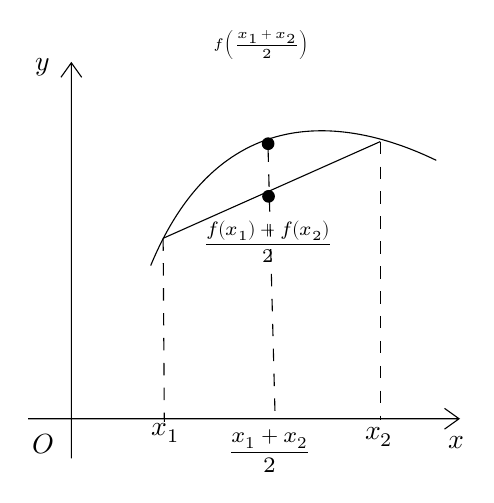
\begin{tikzpicture}[x=0.75pt,y=0.75pt,yscale=-1,xscale=1]
                \draw  (54,203.94) -- (261.57,203.94)(74.76,32.43) -- (74.76,223) (254.57,198.94) -- (261.57,203.94) -- (254.57,208.94) (69.76,39.43) -- (74.76,32.43) -- (79.76,39.43)  ;
                \draw    (113,130.14) .. controls (149,43.29) and (217,63.14) .. (250.57,79.43) ;
                \draw    (119,117) -- (223.57,70.43) ;
                \draw  [dash pattern={on 4.5pt off 4.5pt}]  (119,117) -- (119.57,205.43) ;
                \draw  [dash pattern={on 4.5pt off 4.5pt}]  (223.57,70.43) -- (223.57,204.43) ;
                \draw  [dash pattern={on 4.5pt off 4.5pt}]  (169.57,74.21) -- (173,205.14) ;
                \draw  [color={rgb, 255:red, 0; green, 0; blue, 0 }  ,draw opacity=1 ][fill={rgb, 255:red, 0; green, 0; blue, 0 }  ,fill opacity=1 ] (166.79,71.43) .. controls (166.79,69.89) and (168.03,68.64) .. (169.57,68.64) .. controls (171.11,68.64) and (172.36,69.89) .. (172.36,71.43) .. controls (172.36,72.97) and (171.11,74.21) .. (169.57,74.21) .. controls (168.03,74.21) and (166.79,72.97) .. (166.79,71.43) -- cycle ;
                \draw  [color={rgb, 255:red, 0; green, 0; blue, 0 }  ,draw opacity=1 ][fill={rgb, 255:red, 0; green, 0; blue, 0 }  ,fill opacity=1 ] (167,96.79) .. controls (167,95.25) and (168.25,94) .. (169.79,94) .. controls (171.32,94) and (172.57,95.25) .. (172.57,96.79) .. controls (172.57,98.32) and (171.32,99.57) .. (169.79,99.57) .. controls (168.25,99.57) and (167,98.32) .. (167,96.79) -- cycle ;
                \draw (55,210) node [anchor=north west][inner sep=0.75pt]   [align=left] {$\displaystyle O$};
                \draw (255,211) node [anchor=north west][inner sep=0.75pt]   [align=left] {$\displaystyle x$};
                \draw (56,29) node [anchor=north west][inner sep=0.75pt]   [align=left] {$\displaystyle y$};
                \draw (112,205) node [anchor=north west][inner sep=0.75pt]   [align=left] {$\displaystyle x_{1}$};
                \draw (215,207) node [anchor=north west][inner sep=0.75pt]   [align=left] {$\displaystyle x_{2}$};
                \draw (149,208) node [anchor=north west][inner sep=0.75pt]  [font=\footnotesize] [align=left] {$\displaystyle \dfrac{x_{1} +x_{2}}{2}$};
                \draw (141.79,15.79) node [anchor=north west][inner sep=0.75pt]  [font=\tiny] [align=left] {$\displaystyle f\left(\dfrac{x_{1} +x_{2}}{2}\right)$};
                \draw (136.79,107.57) node [anchor=north west][inner sep=0.75pt]  [font=\scriptsize] [align=left] {$\displaystyle \dfrac{f( x_{1}) +f( x_{2})}{2}$};
            \end{tikzpicture}
        \end{center}
    \end{defn}
    \begin{criterion}{凹凸性注意事项}{}
        \begin{enumerate}
            \item 凹凸性指的是函数区间上的性质,不是一点处的.
        \end{enumerate}
    \end{criterion}
    \begin{defn}{凹凸性的第二种定义(广义定义)}{}
        对于区间$I$上介于任意两点$x_1,x_2$之间的点$tx_1+(1-t)x_2,0\leq t\leq1$,若曲线$y=f(x)$为凹曲线,则
        $$f\left(tx_{1}+\left(1-t\right)x_{2}\right)\leq tf\left(x_{1}\right)+\left(1-t\right)f\left(x_{2}\right)$$
        若曲线 $y=f\left(x\right)$为凸曲线,则
        $$f\left(tx_{1}+\left(1-t\right)x_{2}\right)\geq tf\left(x_{1}\right)+\left(1-t\right)f\left(x_{2}\right)$$
        等号均在$t=0$和$t=1$时取得
    \end{defn}
    \begin{criterion}{凹凸性第二种定义的几何意义}{}
        $y=f(x_0)+f^\prime(x_0)(x-x_0)$是曲线$y=f(x)$在点$(x_0,f(x_0))$处的切线方程,因此该表达式的几何意义如下图所示.若曲线 $y=f(x)(a<x<b)$在任意点处的切线(除该点外)总在曲线的下方(上方),则该曲线是凹(凸)的.
        \begin{center}
            \tikzset{every picture/.style={line width=0.75pt}} %set default line width to 0.75pt        
            \begin{tikzpicture}[x=0.75pt,y=0.75pt,yscale=-1,xscale=1]
                \draw  (54,203.94) -- (261.57,203.94)(74.76,32.43) -- (74.76,223) (254.57,198.94) -- (261.57,203.94) -- (254.57,208.94) (69.76,39.43) -- (74.76,32.43) -- (79.76,39.43)  ;
                \draw    (91,142.14) .. controls (125,98.29) and (188,92.14) .. (235,112.14) ;
                \draw    (360,131.14) .. controls (425,158.14) and (474,141.14) .. (504,101.14) ;
                \draw  (326,204.94) -- (533.57,204.94)(346.76,33.43) -- (346.76,224) (526.57,199.94) -- (533.57,204.94) -- (526.57,209.94) (341.76,40.43) -- (346.76,33.43) -- (351.76,40.43)  ;
                \draw  [dash pattern={on 4.5pt off 4.5pt}]  (91,142.14) -- (91,203.14) ;
                \draw  [dash pattern={on 4.5pt off 4.5pt}]  (235,112.14) -- (235,202.14) ;
                \draw  [dash pattern={on 4.5pt off 4.5pt}]  (360,131.14) -- (361,204.14) ;
                \draw  [dash pattern={on 4.5pt off 4.5pt}]  (504,101.14) -- (505,204.14) ;
                \draw  [dash pattern={on 4.5pt off 4.5pt}]  (168,103.14) -- (168,202.14) ;
                \draw  [dash pattern={on 4.5pt off 4.5pt}]  (431,146.14) -- (432,207.14) ;
                \draw    (86,112.14) -- (260,92.14) ;
                \draw    (344,156.14) -- (518,133.14) ;
                \draw (55,210) node [anchor=north west][inner sep=0.75pt]   [align=left] {$\displaystyle O$};
                \draw (255,211) node [anchor=north west][inner sep=0.75pt]   [align=left] {$\displaystyle x$};
                \draw (56,29) node [anchor=north west][inner sep=0.75pt]   [align=left] {$\displaystyle y$};
                \draw (333,208) node [anchor=north west][inner sep=0.75pt]   [align=left] {$\displaystyle O$};
                \draw (86,208) node [anchor=north west][inner sep=0.75pt]   [align=left] {$\displaystyle a$};
                \draw (357,209) node [anchor=north west][inner sep=0.75pt]   [align=left] {$\displaystyle a$};
                \draw (230,210) node [anchor=north west][inner sep=0.75pt]   [align=left] {$\displaystyle b$};
                \draw (501,212) node [anchor=north west][inner sep=0.75pt]   [align=left] {$\displaystyle b$};
                \draw (159,208) node [anchor=north west][inner sep=0.75pt]   [align=left] {$\displaystyle x_{0}$};
                \draw (423,212) node [anchor=north west][inner sep=0.75pt]   [align=left] {$\displaystyle x_{0}$};
                \draw (243,106) node [anchor=north west][inner sep=0.75pt]   [align=left] {$\displaystyle f( x)$};
                \draw (369,115) node [anchor=north west][inner sep=0.75pt]   [align=left] {$\displaystyle f( x)$};
            \end{tikzpicture}
        \end{center}
    \end{criterion}
    \begin{problem}
    设函数$f(x)$ 具有2阶导数,$g(x)=f(0)(1-x)+f(1)x$,则在区间[0,1]上\\
    (A)当$f^\prime(x)\geqslant0$时$,f(x)\geq g(x).$ \quad (B)当$f^\prime(x)\geqslant0$时$,f(x)\leq g(x).$\\
    (C)当$f^{\prime\prime}(x)\geqslant0$时$,f(x)\geqslant g(x).$ \quad (D)当$f^{\prime\prime}(x)\geqslant0$时$,f(x)\leq g(x).$
    \end{problem}
    \begin{solution}
        根据凹凸性的广义定义,可以观察到二者之间的相似性.当$x_1=1,x_2=0$时,即为:$f(x_2)(1-t)+f(x_1)t$,$t$为自变量,定义域为$[0,1]$.则可以得到$g(x)$为一次函数,并且$g(x)$过$(0,f(0)),(1,f(1))$.根据$D$选项可知,$f^{''}(x)\geqslant0$,则显然$f(x)$为凹函数且$f(x)\leqslant g(x)$
    \end{solution}
    \begin{note}
        本题不太好想,建议使用排除法,排除其他三个选项.
    \end{note}
    \subsubsection{凹凸性的判别}
    \begin{defn}{凹凸性的判别}{}
        设函数$f(x)$在区间上二阶可导:
        \begin{enumerate}
            \item 若在区间上$f^{\prime\prime}(x)>0$,则$f(x)$在区间上的图形是凹的
            \item 若在区间上$f^{\prime\prime}(x)<$0,则$f(x)$在区间上的图形是凸的
        \end{enumerate}
    \end{defn}
    \begin{criterion}{凹凸性判定的注意事项}{}
        \begin{enumerate}
            \item 给出一点的正负值,无法推断出邻域内的凹凸性,因此$f^{''}(x_0)>0\begin{cases}
                          \nRightarrow \text{邻域内}f^{''}(x)>0 \\
                          \nRightarrow \text{邻域内}f(x)\text{为凹函数}
                      \end{cases}$
            \item 函数为凹函数,推不出二阶导大于0,如$f(x)=|x|$(因为凹凸性不是用二阶导去定义的.而且一点处的二阶导推不出凹凸性)
            \item 在第二个注意事项的基础上,即使增加条件:"$f(x)$二阶连续可导,且函数为凹函数",也推不出二阶导大于0\footnote{二阶导大于0,可推出是凹函数},如$f(x)=x^4$,显然为凹函数,但0点处二阶导等于0.(可能二阶导等于0的点)
        \end{enumerate}
    \end{criterion}
    \subsection{拐点}
    \subsubsection{拐点的定义}
    \begin{defn}{拐点的定义}{}
        连续曲线的凹弧与凸弧的分界点称为该曲线的拐点
    \end{defn}
    \begin{criterion}{拐点存在的情况}{}
        若点$(x_0,f(x_0))$为曲线 $y=f(x)$的拐点,则只有以下两种情况
        \begin{enumerate}
            \item $f^{\prime\prime}\left(x_{0}\right)=0$,如 $y=x^{3}$ 在$\left(0,0\right)$处的情形
            \item $f^{\prime\prime}(x_0)$不存在,如$y=\sqrt[3]{x}$在$(0,0)$处的情形
        \end{enumerate}
    \end{criterion}
    \subsubsection{拐点的判别}
    \begin{defn}{拐点的判别的必要条件}{}
        设$f^{\prime\prime}(x_0)$存在,且点$(x_0,f(x_0))$为曲线的拐点,则$f^{\prime\prime}(x_0)=0$
    \end{defn}
    \begin{defn}{拐点的判别的第一充分条件}{}
        设$f(x)$在点 $x=x_0$处连续,在点 $x=x_0$的某去心邻域$\mathring U(x_0,\delta)$内二阶导数存在,且在该点的左、右邻域内$f^{\prime\prime}(x)$变号 (无论是由正变负,还是由负变正 ),则点 $(x_0,f(x_0))$为曲线的拐点\footnote{$(x_0,f(x_0))$为曲线$y=f(x)$的拐点,并不要求$f(x)$在点$x_0$的导数存在}.
    \end{defn}
    \begin{defn}{拐点的判别的第二充分条件}{}
        设$f(x)$在 $x=x_0$ 的某邻域内三阶可导,且$f^{\prime\prime}(x_0)=0,f^{\prime\prime\prime}(x_0)\neq0$,则点$(x_0,f(x_0))$为曲线的拐点.
    \end{defn}
    \textbf{在拐点判断时优先考虑第二充分条件.}
    \begin{defn}{拐点的判别的第三充分条件}{}
        设$f(x)$在$x_0$处$n$ 阶可导,且$f^{(m)}(x_0)=0(m=2,\cdots,n-1),f^{(n)}(x_0)\neq0(n\geqslant3)$,则当$n$为奇数时,点$(x_0,f(x_0))$为曲线的拐点
    \end{defn}
    需要注意的是,拐点判断的三个充分条件都对$f'(x)$无要求,只要求了更高阶的导数.
    \begin{conclusion}{极值点和拐点的重要结论}{}
        \begin{enumerate}
            \item 极值点的必要和三个充分条件中的导数提高一阶就是拐点的必要条件和三个充分条件
            \item \textcolor{red}{若$f(x)$在某点去心邻域内可导\footnote{可以不可导,但是必须有定义},则极值点为去心邻域内导数变号\footnote{函数单调性发生改变}的点}.
            \item \textcolor{red}{若$f(x)$在某点去心邻域内二阶可导\footnote{此点二阶导可以不存在,但是必须有定义},则拐点为去心邻域内二阶导变号\footnote{一阶导单调性发生改变}的点.}
            \item 关于极值点和拐点的第三充分条件,可以通过举特殊例子来进行使用
                  \begin{itemize}
                      \item $n=2$时,一阶导等于0,二阶导不为0,该点为极值点
                      \item $n=3$时,二阶导等于0,三阶导不为0,该点为拐点
                  \end{itemize}
            \item 曲线的可导点不可同时为极值点和拐点;曲线的不可导点可同时为极值点和拐点
            \item 设多项式函数$f(x)=(x-a)^n g(x)(n>1)$,且$g(a)\neq0$,则当$n$为偶数时,$x=a$是$f(x)$的极值点;当$n$为奇数时,点$(a,0)$是曲线$f(x)$的拐点.
            \item 设多项式函数$f(x)=(x-a_1)^{n_1}(x-a_2)^{n_2}...(x-a_k)^{n_k}$,其中$n_i$是正整数,$a_i$是实数且$a_i$两两不等,$i= 1, 2, \cdots,k$.记$k_1$为$n_i=1$ 的个数,$k_2$为$n_i>1$且$n_i$为偶数的个数,$k_3$为$n_i>1$且$n_i$为奇数的个数,则$f(x)$的极值点个数为$k_1+2k_2+k_3-1$,拐点个数为$k_1+2k_2+3k_3-2.$
        \end{enumerate}
    \end{conclusion}
    \begin{problem}
    设函数 $y=\left|x\mathrm{e}^{-x}\right|$,则\\
    $(A)x=0$ 是 $y$ 的极大值点,点$(0,0)$ 不是曲线 $y$ 的拐点\\
    $(B)x=0$ 是 $y$ 的极小值点,点$(0,0)$ 不是曲线 $y$ 的拐点\\
    $(C)x=0$ 是 $y$ 的极大值点,点$(0,0)$ 是曲线 $y$ 的拐点\\
    $(D)x=0$ 是 $y$ 的极小值点,点$(0,0)$ 是曲线 $y$ 的拐点
    \end{problem}
    \begin{solution}
        对函数求一阶导数:$y'=\begin{cases}\mathrm{e}^{-x}\left(x-1\right),&x<0,\\\mathrm{e}^{-x}\left(1-x\right),&x>0.\end{cases}$,求一阶导数的左右极限,易知该点两侧极限不相等,因此该点不可导. 对该点求二阶导可得: $y''=\begin{cases}\mathrm{e}^{-x}(2-x),&x<0\\\mathrm{e}^{-x}(x-2),&x>0\end{cases}.$此外,易知$f(0)=0$,那么该点必为函数极值点,当$x<0$时,$y''=\mathrm{e}^{-x}(2-x)>0;$当$0<x<2$时,$y''=\mathrm{e}^{-x}(x-2)<0$,可知$y''$在$x=0$的左、右邻域内符号不同.因此点 (0,0)为曲线$y$的拐点.
    \end{solution}
    \begin{note}
        本题易忽视$(0,0)$是函数的不可导点,进而无法判断出该点的极值性和是否为拐点.其次还有一个易被忽视的是,曲线的不可导点可同时为极值点和拐点.还有就是忽略了极值/拐点存在的第二充分条件并非充要条件.
    \end{note}
    \begin{problem}
    设 $f(x)$有二阶连续导数,且$f^{\prime}(0)=0,\operatorname*{lim}_{x\to0}\dfrac{f^{\prime\prime}(x)}{|x|}=1$,则\\
    $(A)f(0)$是$f(x)$的极大值.\quad
    $(B)f(0)$是$f(x)$的极小值.\\
    $(C)(0,f(0))$是曲线$y=f(x)$的拐点.\quad
    $(D)f(0)$不是$f(x)$的极值,$(0,f(0))$也不是曲线$y=f(x)$的拐点.
    \end{problem}
    \begin{solution}
        已知$\lim_{x\to 0}\dfrac{f^{''}(x)}{|x|}=1$,$x\to 0$时$|x|$大于0,则$f''(x)$在0邻域内也大于0,又因为$f'(0)=0$,则显然$f(0)$为$f(x)$的极小值点.综上,应当选择B选项.
    \end{solution}
    \begin{problem}
    \getRating{1}设$y=f(x)$在$(-\infty,\infty)$上连续,且其导函数$f^{\prime}(x)$ 的图形如图所示,其中$x=0$和$x=x_5$是$f^\prime(x)$的铅直渐近线,则$y=f(x)$极值点的个数为().拐点的个数为()
    \begin{center}
        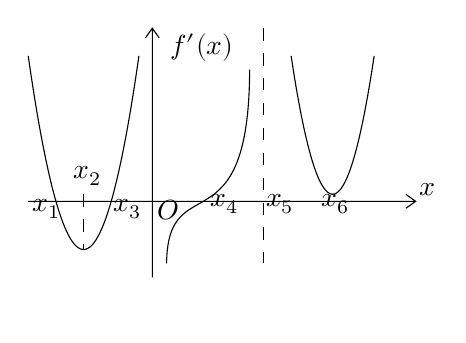
\begin{tikzpicture}[x=0.5pt,y=0.5pt,yscale=-1,xscale=1]
            \draw  (30,205.1) -- (310,205.1)(119.67,80) -- (119.67,260) (303,200.1) -- (310,205.1) -- (303,210.1) (114.67,87) -- (119.67,80) -- (124.67,87)  ;
            \draw   (30,100) .. controls (56.67,286.67) and (83.33,286.67) .. (110,100) ;
            \draw  [dash pattern={on 4.5pt off 4.5pt}]  (70,200) -- (70,240) ;
            \draw    (130,250) .. controls (130.67,179) and (189.67,242) .. (190,110) ;
            \draw  [dash pattern={on 4.5pt off 4.5pt}]  (200,80) -- (200,250) ;
            \draw   (220,100) .. controls (240,233.33) and (260,233.33) .. (280,100) ;
            \draw (311.18,189.89) node [anchor=north west][inner sep=0.75pt]  [rotate=-0.51] [align=left] {$\displaystyle x$};
            \draw (131,82) node [anchor=north west][inner sep=0.75pt]   [align=left] {$\displaystyle f'( x)$};
            \draw (31,202) node [anchor=north west][inner sep=0.75pt]   [align=left] {$\displaystyle x_{1}$};
            \draw (61,178) node [anchor=north west][inner sep=0.75pt]   [align=left] {$\displaystyle x_{2}$};
            \draw (90,202) node [anchor=north west][inner sep=0.75pt]   [align=left] {$\displaystyle x_{3}$};
            \draw (160,198) node [anchor=north west][inner sep=0.75pt]   [align=left] {$\displaystyle x_{4}$};
            \draw (200,198) node [anchor=north west][inner sep=0.75pt]   [align=left] {$\displaystyle x_{5}$};
            \draw (240,198) node [anchor=north west][inner sep=0.75pt]   [align=left] {$\displaystyle x_{6}$};
            \draw (121.67,202) node [anchor=north west][inner sep=0.75pt]   [align=left] {$\displaystyle O$};
        \end{tikzpicture}
    \end{center}
    \end{problem}
    \begin{solution}
        根据极值点和拐点的第一充分条件,去心邻域内导数变号的点是极值点,则从图中可以观察到去心邻域内变号的点为$x_1,x_3,O,x_4$.拐点为二阶导变号的点,那么一阶导的单调性在此邻域内应发生改变,从图中可以观察到$x_2,x_6,x_5$.综上所示,$f(x)$的极值点个数为4个,拐点的个数为3个.
    \end{solution}
    \begin{problem}
    曲线$y=(x-1)(x-2)^2(x-3)^3(x-4)^4$的拐点是\\
    A:(1,0) \quad B:(2,0) \quad C:(3,0) \quad D:(4,0)
    \end{problem}
    \begin{solution}
        根据$f(x)$的$n$重根的特性,$f'(3)=f''(3)=0,f^{'''}(3)\neq0$,根据拐点第二充分条件,则该点为$f(x)$的拐点.综上,应当选择C选项.
    \end{solution}
    \begin{note}
        对于其他选项,BD可以通过拐点的第二充分条件和 $n$重根的性质判断出正确性.但是对于$(1,0)$,无法通过上述判断方法来判断.因为第二充分条件只要求了二阶和三阶导数,没有要求一阶导数,因此$(1,0)$无法判断出.那么如果想判断出该点是否为拐点,只能通过定义来判断.则$f'(x)=g(x)+(x-1)g'(x),f''(x)=2g'(x)+(x-1)g''(x)$,代入$x=1$得:$f''(1)\neq0$,则该点不为拐点.此外,本题还可以使用初中的穿针引线法,但是不建议使用这个方法,因为无法判断出具体的凹凸性,只能排除错误选项.
    \end{note}
    \begin{conclusion}{关于$f(x)$的$n$重根}{}
        设$x_0$是方程$f(x)=0$的$n$重根,即$f(x)=(x-x_0)^ng(x)$且$g(x_0)\neq0.$若$g(x)$具有$n$阶导数,则
        \begin{enumerate}
            \item 当$n=1$时,$f^\prime(x_0)\neq0$,即$x_0$不是$f^\prime(x)=0$的根
            \item 当$n\geqslant2$时,$x_0$是$f^\prime(x)=0$ 的$n-1$ 重根.依此类推$,x_0$ 是$f^{(k)}(x)=0$ 的$n-k$ 重根$,k=1,2,\cdots,n-1$,且 $x_0$ 不是$f^{(n)}(x)=0$ 的根
        \end{enumerate}
        上述结论可简单表述为,求一次导,根的重数减少一次.
    \end{conclusion}
    \begin{problem}
    设函数$f(x)$有二阶导数,且$\operatorname*{lim}_{x\to0}\dfrac{f(x)-a}{\operatorname{ln}(1+x)}=0\,,\operatorname*{lim}_{x\to0}\dfrac{f^{\prime\prime}(x)-1}{\mathrm{e}^{x^{2}}-1}=2021$,则\\
    (A)$f(0)$是$f(x)$的极大值.\quad
    (B)$f(0)$是$f(x)$的极小值.\\
    (C)$(0,f(0))$是曲线$y=f(x)$的拐点.\quad
    (D)$f(0)$不是$f(x)$的极值,$(0,f(0))$也不是曲线$y=f(x)$的拐点.
    \end{problem}
    \begin{solution}
        已知
        \begin{align*}
            \operatorname*{lim}_{x\to0}\dfrac{f(x)-a}{\operatorname{ln}(1+x)} & = \lim_{x\to 0}\dfrac{f(x)-a}{x}        \\
                                                                              & = \lim_{x\to 0}\dfrac{f'(x)}{1}=f'(0)=0
        \end{align*}
        \begin{align*}
            \operatorname*{lim}_{x\to0}\dfrac{f^{\prime\prime}(x)-1}{\mathrm{e}^{x^{2}}-1} & =  \lim_{x\to 0}\dfrac{f''(x)-1}{x^2} \\
                                                                                           & = \lim_{x\to 0} f''(x) \to 1          \\
                                                                                           & =f''(0)=1
        \end{align*}
        由上述条件根据极值点的第二充分条件可得:$x=0$为极小值点.
    \end{solution}
    \subsection{曲率与曲率半径}
    \begin{defn}{曲率与曲率半径的计算公式}{}
        曲率的定义为
        $$
            k=\lim_{\Delta s\to0}\left|\frac{\Delta\alpha}{\Delta s}\right|
        $$
        设$y(x)$二阶可导,则曲线$y=y(x)$在点$(x,y(x))$处的曲率公式为
        $$
            k=\dfrac{\left|y^{\prime\prime}\right|}{\left[1+(y^{\prime})^2\right]^{\frac{3}{2}}}
        $$
        \tcblower
        曲率半径的计算公式
        $$
            R=\dfrac{1}{k}=\dfrac{\left[1+(y')^2\right]^{\frac{3}{2}}}{\left|y''\right|}(y''\neq0)
        $$
    \end{defn}
    曲率是用于描述曲线弯曲程度的量.越大说明曲线越弯曲.
    \begin{problem}
    曲线 $2y^3-2y^2+2xy-x^2=1$ 在$(1,1)$ 处的曲率半径为
    \end{problem}
    \begin{solution}
        对曲线中变量$x$求一阶导数和二阶导数可得:$6y^2y'-4yy'+2y+2xy'-2x=0$,$(6yy^{\prime}-2y^{\prime}+1)y^{\prime}+(3y^{2}-2y+x)y^{\prime\prime}+y^{\prime}-1=0$,代入$(1,1)$可得$y'(1)=0,y''(1)=\dfrac{1}{2}$.
        代入$k=\dfrac{\left|y^{\prime\prime}\right|}{\left[1+(y^{\prime})^2\right]^{\frac{3}{2}}}$可得$k=\dfrac{1}{2}$,曲率$R=2.$
    \end{solution}
    \begin{problem}
    对数曲线 $y=\ln x$ 在点 $P$ 处的曲率半径最小,则该最小半径是
    \end{problem}
    \begin{solution}
        设$P(x,\operatorname{ln}x),x>0$,曲率半径
        $$
            R=\dfrac{\left[1+(y^{\prime})^{2}\right]^{\frac{3}{2}}}{\mid y^{\prime\prime}\mid}=\dfrac{(1+x^{2})^{\frac{3}{2}}}{x},x>0
        $$
        令$R^{\prime}={\dfrac{(1+x^{2})^{\frac{1}{2}}(2x^{2}-1)}{x^{2}}}=0$,得唯一驻点$x={\dfrac{\sqrt{2}}{2}}$.于是$y=\operatorname{ln}x$在点$\left({\dfrac{\sqrt{2}}{2}},-{\dfrac{\operatorname{ln}2}{2}}\right)$的曲率半径最小,此最小收敛半径$R={\dfrac{3\,{\sqrt{3}}}{2}}$
    \end{solution}
    \begin{problem}
    \getRating{1}已知$f(x),g(x)$ 2阶可导且2阶导函数在$x=a$处连续,则$\lim_{x\to a} \dfrac{f(x)-g(x)}{\left(x-a\right)^2}=0$是曲线$y=f(x)$和$y=g(x)$在$x=a$对应的点处相切且曲率相等的()\\
    (A) 充分非必要条件.\quad (B) 充分必要条件.\quad (C)必要非充分条件.\quad (D) 既非充分又非必要条件.
    \end{problem}
    \begin{solution}
        因为$f(x),g(x)$二阶可导且二阶导函数在$x=a$处连续,根据带佩亚诺余项的泰勒展开式可得$f(x)=f(a)+f^{\prime}(a)(x-a)+\dfrac{f^{\prime\prime}(a)}{2}(x-a)^{2}+o((x-a)^{2}),g(x)=g(a)+g^{\prime}(a)(x-a)+\dfrac{g^{\prime\prime}(a)}{2}(x-a)^{2}+o((x-a)^{2}).$将其代入$\lim_{x\to a} \dfrac{f(x)-g(x)}{\left(x-a\right)^2}=0$可得
        $$
            \lim_{x\to a}\dfrac{f(x)-g(x)}{\left(x-a\right)^{2}}=\lim_{x\to a}\dfrac{f(a)-g(a)+f'(a)-g'(a)(x-a)+\dfrac{f''(a)-g''(a)}{2}(x-a)^{2}+o((x-a)^{2})}{\left(x-a\right)^{2}}=0
        $$
        由上式可知$\lim\limits_{x\to a}\dfrac{f(x)-g(x)}{\left(x-a\right)^2}=0$当且仅当$\begin{cases}f(a)=g(a)\\f'(a)=g'(a)\\f''(a)=g''(a)\end{cases}$.由上述条件推断$f(x)$与$g(x)$在$x=a$处的关系,显然在$x=a$点,二者相切且曲率相等.因此$\lim_{x\to a} \dfrac{f(x)-g(x)}{\left(x-a\right)^2}=0$是曲线$y=f(x)$和$y=g(x)$在$x=a$对应的点处相切且曲率相等的充分条件.但是反过来,由于$k=\dfrac{\left|y^{\prime\prime}\right|}{\left[1+(y^{\prime})^2\right]^{\frac{3}{2}}}$,则$|f''(a)|=|g''(a)|$,无法得到相关结论.综上所示$\lim_{x\to a} \dfrac{f(x)-g(x)}{\left(x-a\right)^2}=0$是曲线$y=f(x)$和$y=g(x)$在$x=a$对应的点处相切且曲率相等的充分条件不必要条件.
    \end{solution}
    \begin{problem}
    若$f^{\prime\prime}(x)$ 不变号,且曲线 $y=f(x)$ 在点$(1,1)$处的曲率圆为 $x^2+y^2=2$,则函数$f(x)$在区间$(1,2)$内()\\
    (A)有极值点,无零点\quad(B)无极值点,有零点\quad(C)有极值点,有零点\quad(D) 无极值点,无零点
    \end{problem}
    \begin{solution}
        由于曲线$y=f(x)$ 在点$(1,1)$处的曲率圆为 $x^2+y^2=2$,则可以用曲率圆来近似该点方程.对曲率圆方程进行$x$变量求导得$2x+2yy'=0$,再次求导得$2+2(y')^2+2yy'=0$.代入$x=1,y(1)=1$得$y'(1)=-1,y''(-1)=-2.$由于$f''(x)$不变号,则$y''$在$(1,2)$上恒小于0.综上$f(x)$在区间上无极值点.根据题设条件$f(1)>0$,现在只需要判断$f(2)$的正负即可.已知$f(x)$在区间上单减,则根据拉格朗日中值定理\footnote{看见导数和函数就要想到拉格朗日中值定理}可得:$f(2)-f(1)=f'(\xi )=f'(\xi)+1$,由于$f^\prime(x)$在$(1,2)$上单调减少,且$f^\prime(1)=-1$,从而$f^\prime(\xi)<-1$,故$f(2)=1+f^\prime(\xi)<0.$ 因为$f(1)=1>0,f(2)<0$,所以由连续函数的介值定理知$,f(x)$ 在(1,2)上存在零点.综上,应当选择B选项.
    \end{solution}
    \begin{criterion}{曲率圆的作用}{}
        由于曲线$y=f(x)$在某点的曲率圆与曲线在该点具有相同的切线和曲率,且在该点附近具有相同的凹凸性.则在实际问题中,\textbf{常用曲率圆在点 $M$ 附近的一段圆弧来近似代替曲线弧使问题简化}.
    \end{criterion}
    \subsection{渐近线}
    \subsubsection{铅直渐近线}
    \begin{defn}{铅直渐近线定义}{}
        若$\lim_{x\to x_0^+}f(x)=\infty($或$\lim_{x\to x_0^-}f(x)=\infty)$,则$x=x_0$为一条铅直渐近线.
    \end{defn}
    \subsubsection{水平渐近线}
    \begin{defn}{水平渐近线定义}{}
        若$\lim_{x\to+\infty} f(x)=y_{1}$,则$y=y_1$为一条水平渐近线.\\
        若$\lim_{x\to-\infty} f(x)=y_{2}$,则$y=y_{2}$为一条水平渐近线.\\
        若$\lim _{x\to + \infty }f( x) = \lim _{x\to - \infty }f( x) = y_{0}$ , 则 $y= y_{0}$为一条水平渐近线
    \end{defn}
    \subsubsection{斜渐近线}
    \begin{defn}{斜渐近线定义}{}
        若$\lim_{x\to+\infty}\dfrac{f(x)}{x}=a_{1}(a_{1}\neq0),\lim_{x\to+\infty}\Big[f(x)-a_{1}x\Big]=b_{1}$,则$y=a_{1}x+b_{1}$是曲线$y=f(x)$的一条斜渐近线\\
        若$\lim\limits_{x\to-\infty}\dfrac{f(x)}{x}=a_2(a_2 \neq 0),\lim\limits_{x\to-\infty}\left[f(x)-a_2x\right]=b_2$,则$y=a_2x+b_2$是曲线$y=f(x)$的一条斜渐近线\\
        若$\lim_{x\to+\infty} \dfrac{f(x)}x=\lim_{x\to-\infty}\dfrac{f(x)}x=a(a\neq0),\lim_{x\to+\infty}\left[f(x)-ax\right]=\lim_{x\to-\infty}\left[f(x)-ax\right]=b,则y=ax+b$是曲线$y=f(x)$的一条斜渐近线.
    \end{defn}
    \begin{problem}
    曲线 $y=\dfrac{(1+x)^{\frac32}}{\sqrt x}$的斜渐近线方程为
    \end{problem}
    \begin{solution}
        $\lim_{x\to +\infty}\dfrac{y}{x}=\lim_{x\to+\infty}\dfrac{(1+x)^{\frac{3}{2}}}{x^{\frac{3}{2}}}=\lim_{x\to +\infty}(1+\dfrac{1}{x})^{\frac{3}{2}}=1=k$\\
        $\lim_{x\to +\infty}(y-kx)=\lim_{x\to +\infty}\dfrac{(1+x)^{\frac{3}{2}}}{\sqrt{x}}-x=\lim_{x\to +\infty}\dfrac{(1+x)^{\frac{3}{2}}-x\sqrt{x}}{\sqrt{x}}=\lim_{x\to +\infty}\dfrac{x^{\frac{3}{2}}[(1+\dfrac{1}{x})^{\frac{3}{2}}-1]}{\sqrt{x}}=\lim_{x\to+\infty}\dfrac{x^{\frac32}\cdot\dfrac32\cdot\dfrac1x}{\sqrt{x}}=\dfrac{3}{2}=b$\\
        综上,斜渐近线方程为$y=x+\dfrac{3}{2}$
    \end{solution}
    \begin{problem}
    曲线$y=\mathrm{e}^{x+\frac1x}\arctan\dfrac{x^2+x+1}{(x-1)(x-2)}$的渐近线条数是
    \end{problem}
    \begin{solution}
        由于$\operatorname*{lim}_{x\to0^{+}}\mathrm{e}^{x+\frac{1}{x}}\operatorname{arctan}\dfrac{x^{2}+x+1}{(x-1)\left(x-2\right)}=+\infty$,则$x=0$为其铅直渐近线\\
        由于$\operatorname*{lim}_{x\to-\infty}\mathrm{e}^{x+\frac{1}{x}}\mathrm{arctan}\,\dfrac{x^{2}+x+1}{(x-1)\,(x-2)}=0$,则$y=0$水平渐近线.\\
        由于$\operatorname* {l i m}_{x \to+\infty} {\dfrac{y} {x}}=\operatorname* {l i m}_{x \to+\infty} {\dfrac{\mathrm{e}^{x}} {x}} \mathrm{e}^{\frac{1} {x}} \arctan{\dfrac{x^{2}+x+1} {\left( x-1 \right) \left( x-2 \right)}}=+\infty$(不存在),则原曲线无斜渐近线\\
        综上,曲线的渐近线个数为3个.
    \end{solution}
    \begin{note}
        在判断渐近线条数时,需要判断$x\to \text{无定义点}$(可能出现铅直渐近线)和$x\to \text{无穷}$(可能出现水平渐近线,斜渐近线)
    \end{note}
    \begin{problem}
    求函数 $y=( x-1 ) \mathrm{e}^{\frac{\pi} {2}+\arctan x}$渐近线
    \end{problem}
    \begin{solution}
        $k=\lim_{x\to+\infty}\dfrac{y}{x}=\lim_{x\to+\infty}\dfrac{(x-1)e^{\frac{\pi}{2}+\arctan x}}{x}=e^\pi$\\
        $b=(y-kx)=(x-1)e^{\frac{\pi}{2}+\arctan x}-e^\pi x=e^\pi+\lim_{x\to +\infty}x(e^{\frac{\pi}{2}+\arctan x}-e^\pi) $\\
        此后有三种解法:\\
        (1)拉格朗日中值定理:
        \begin{align*}
            \text{原式} & = \lim_{x\to +\infty}x\times e^{(\varepsilon)}(\arctan x -\dfrac{\pi}{2}) \\
                      & = e^{\pi} \lim_{x\to +\infty}\dfrac{\arctan x -\dfrac{\pi}{2}}{\dfrac1x}  \\
                      & =\lim_{x\to +\infty} \dfrac{\dfrac{1}{1+x^2}}{-\dfrac{1}{x^2}}            \\
                      & =-e^\pi
        \end{align*}
        (2)提后项:
        \begin{align*}
            \text{原式} & = \lim_{x\to +\infty}e^\pi(e^{\arctan \frac{\pi}{2}}-1) \\
                      & =\lim_{x\to +\infty}e^\pi\times\arctan \frac{-\pi x}{2} \\
                      & =-e^\pi
        \end{align*}
        (3)直接洛:
        \begin{align*}
            \text{原式} & = \lim_{x\to +\infty}\frac{e^{\frac{\pi+\arctan x}{2}}-e^\pi}{\frac{1}{x}}       \\
                      & = \dfrac{e^{\frac{\pi}{2}+\arctan x}\times\dfrac{1}{1+x^{2}}}{-\dfrac{1}{x^{2}}} \\
                      & = -e^\pi
        \end{align*}
        综上,渐近线方程为$y=e^\pi x-2e^\pi.$
    \end{solution}
    \begin{note}
        渐近线的考察点主要在于斜进线,斜渐近线的求解主要在无穷减无穷上.
    \end{note}
    \begin{problem}
    已知$\int_{0}^{+\infty} \mathrm{e}^{-t^{2}} \mathrm{d} t={\dfrac{\sqrt{\pi}} {2}}$ ,求曲线 $y=( 5 x+9 ) \int_{0}^{-x} \mathrm{e}^{-t^{2}} \mathrm{d} t+( 7 x-3 ) \int_{0}^{x} \mathrm{e}^{-t^{2}} \mathrm{d} t$ 的斜渐近线方程
    \end{problem}
    \begin{solution}

    \end{solution}
    \begin{problem}
    求曲线 $y=\sqrt{4x^2+x}\ln\left(2+\dfrac1x\right)$的全部渐近线.
    \end{problem}
    \begin{solution}

    \end{solution}
    \begin{problem}
    求曲线 $y= \dfrac {x^{1+ x}}{\left ( 1+ x\right ) ^{x}}( x >0)$ 的斜渐近线方程.
    \end{problem}
    \begin{solution}
        % //TODO
    \end{solution}
    \subsection{方程根的个数}
    %  ############################ 正文部分
    \ifx\allfiles\undefined
\end{sloppypar}
\end{document}
\fi
